\documentclass[12pt, chapterprefix=true]{scrreprt}

%packages
\usepackage[utf8]{inputenc}
\usepackage{mathtools}
\usepackage{amsfonts}
\usepackage{pifont}
\usepackage[onehalfspacing]{setspace}
\usepackage{float}
\usepackage{graphicx}
\usepackage[font={small,it}]{caption}
\usepackage{subcaption}
\usepackage[hidelinks]{hyperref}
\usepackage[section]{glossaries}
\usepackage[square]{natbib}

\setkomafont{disposition}{\normalfont\bfseries}
\renewcommand{\baselinestretch}{1.5}

\makeglossaries
%<glossary>
\newglossaryentry{admixture}{
  name=admixture,
  description={Here, genetic admixture. Introduction of new genetic lineages into a population. Refers to the proportion of the genome coming from one ancestral population or another. In the whole context of this project, when talking about admixture, Asian admixture is implied, with a value of one for a completely Asian person, and zero for a person having absolutely no Asian SNPs, and since only two populations are considered, completely Melanesian}
}
\newglossaryentry{deme}{
  name=deme,
  description={Generic name for a single unit of space corresponding to a populated area. This can be assumed similar to a village}
}
\newglossaryentry{job-scheduler}{
  name=job scheduler,
  description={Application used to manage and launch a set of jobs, usually on multiple computers organised as nodes of a cluster, and regulating the amount of work each node is doing at every moment}
}
\newglossaryentry{posterior}{
  name=posterior,
  description={In the context of an ABC statistical analysis, a resulting parameter distribution}
}
\newglossaryentry{prior}{
  name=prior,
  description={In the context of an ABC statistical analysis, an input parameter distribution}
}
%</glossary>

%document
\begin{document}
\begin{titlepage} 
  \parindent0pt 
  \hskip.25cm \vrule width.8pt \hskip.25cm 
  \begin{minipage}{\dimexpr\linewidth*2-2.5cm-.8pt-2.5cm\relax} 
    \sffamily\bfseries {
    \huge Master 2 Bioinformatique\par}\large 
    Semestre 10\par Université de Bordeaux\par 
    %%Année truc
  \end{minipage}%
  \vskip10pt plus 1fil
  \fbox{%
  \begin{minipage}{\dimexpr\linewidth-2\fboxsep-2\fboxrule} 
    \centering\Large\bfseries 
    \vskip1cm 
    Project report: Statistical Analysis Pipeline for Admixture Data from a Human Population Settlement Model\par 
    \vskip1cm \kern0pt 
  \end{minipage}%
  }%
  \vskip0.5cm 
  {\centering 
  \vskip0pt plus 1fil 
  }%

  \LARGE
  Aurélien \textsc{Luciani}\centering\\
  \normalsize
  \vskip0pt plus 1fil 
  \hfill \hskip.25cm \vrule width.8pt \hskip.25cm 
  \vskip0pt plus 1fil {\centering Supervisor: Murray P. \textsc{Cox} \par }
  \vskip0pt {\centering Host: Institute of Fundamental Sciences, Massey University \par }
  \vskip0pt plus 1fil {\centering Université de Bordeaux supervisor: Marie Noelle \textsc{Beurton-Aimar} \par }
  \vskip0pt plus 2fil 
  
\includegraphics[width=0.45\textwidth]{../data/ub.jpg}
  
\includegraphics[width=0.45\textwidth]{../data/mu.png}
  \vskip0pt plus 2fil 
  \hfill\bfseries{Year 2014-2015}\hfill\null 
\end{titlepage}

\clearpage\thispagestyle{empty}\null\newpage

\begin{spacing}{1.21}
\tableofcontents
\end{spacing}
%\addtocontents{toc}{\protect\enlargethispage{\baselineskip}}

\clearpage\thispagestyle{empty}\null\newpage

\chapter*{Acknowledgements}
Special thanks to:
\begin{itemize}
  \item Dr Murray Cox, as the main supervisor of this project and of this internship;
  \item François Vallée, as the research assistant for this project, and developer of the model;
  \item Dr Marie Noelle Beurton-Aimar, as the Université de Bordeaux supervisor of this internship; \textit{and}
  \item all the Computational Biology Research Group, Dr Matthew “Mac” Campbell, Dr Pierre-Yves Dupont, Dr Elsa Guillot, and Jiří Moravec, for the help provided during this internship.
\end{itemize}

Computational Biology Research Group: \url{http://massey.genomicus.com}

\begin{figure}[H]
	\centering
	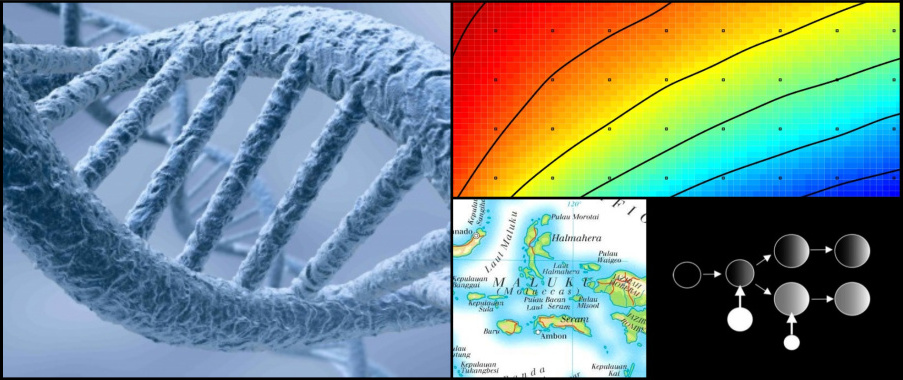
\includegraphics[width=0.7\textwidth]{../data/cbrg.jpg}
\end{figure}

This work is founded by the Rutherford Foundation Trust, part of the Royal Society of New Zealand.
It is hosted at the Institute of Fundamental Sciences (IFS), Massey University, Palmerston North, New Zealand.

\newpage
\newpage

\chapter*{Introduction}
\addcontentsline{toc}{chapter}{Introduction}
Two main ancestral populations can be identified in the genomes of people living nowadays in the Islands of South-East Asia (ISEA).
The first one is the Melanesian population, whose settlement in this area is believed to have taken place around 45 thousand years ago.
The other arrived more recently, during a period often called the Austronesian expansion, between 5 and 4 thousand years ago, when people from what is now mainland China settled in the islands.
This expansion implied great changes for the people living in the islands, including the development of rice agriculture and better navigation knowledge.
The exact path these populations followed is unclear though, and it is believed they might have come through Taiwan, the Malay Peninsula, or from both places around the same time.

Nowadays, people living in this area have mixed genomic ancestry and markers can be identified as either from Asian or Melanesian ancestry.
These markers are based on single nucleotide polymorphisms (SNPs) located on different chromosomes and 37 markers can be used to define accurately the \gls{admixture} of the Asian ancestry in every individual (\cite{Cox01}).
The choice of this set of SNPs is the result of previous studies and the resulting set is defined as highly informative. With this, the ancestry of a person can be defined based on a small quantity of markers that are highly discriminant.

Two specific patterns can be seen (\cite{Lan01}).
One is the non-linear gradient of Asian \gls{admixture} along the longitudinal axis in the different islands in the area, that could correspond more or less to how the Austronesian expansion wave propagated from the mainland.
The second is the difference of \gls{admixture} when looking at specific parts of the genomes associated with male or female ancestry, implying a gender-biased expansion.

These are based on data coming from studies made on population currently living in the ISEA.
These studies were made jointly at Massey University (New Zealand), the University of Arizona (USA), the Santa Fe Institute (USA), and the Eijkman Institute (Indonesia).
They provided the set of SNPs used, determined after the genotyping of 1,430 individuals from 60 populations.
The data and discoveries made led to further questions, such as explaining the different \gls{admixture} patterns.

The Computational Biology Research Group at Massey University (Manawat\={u} campus, in Palmerston North) is doing a follow-up two-year project.
It consists of developing a model of the Austronesian expansion throughout the ISEA that could reproduce the same two patterns observed in the real data.

\chapter{Project presentation}
The scope of this six-month internship is to create a statistical framework to handle the data created by the model.

As the model is currently being implemented in the same research group, the first thing to do is to assess the quality of the model by looking at the returned data.
This is done to guide the development of the model to have the best implementation possible.

Once the model implementation is stable, it can be run to provide data for the statistical analysis. The final goal is thus to compare the simulated data to the reference data, from the previous papers, and to find the same patterns observed with the reference data in the simulations.

This project will need to take into account what is already done to evaluate simulation data and to adapt it to this specific model in order to handle transparently all the simulation data generated.

The first of the two observed patterns can be seen in Figure \ref{cox-image}.
It is a non-linear gradient in Asian \gls{admixture} that declines abruptly around the eastern part of Indonesia.
The second one, represented in Figure \ref{lansing-image}, shows the difference in \gls{admixture} on distinct parts of the DNA for different islands.
These latter differences would tend to appear in a context where marriages between Asian women and Melanesian men would be favoured.

\begin{figure}[H]
	\centering
	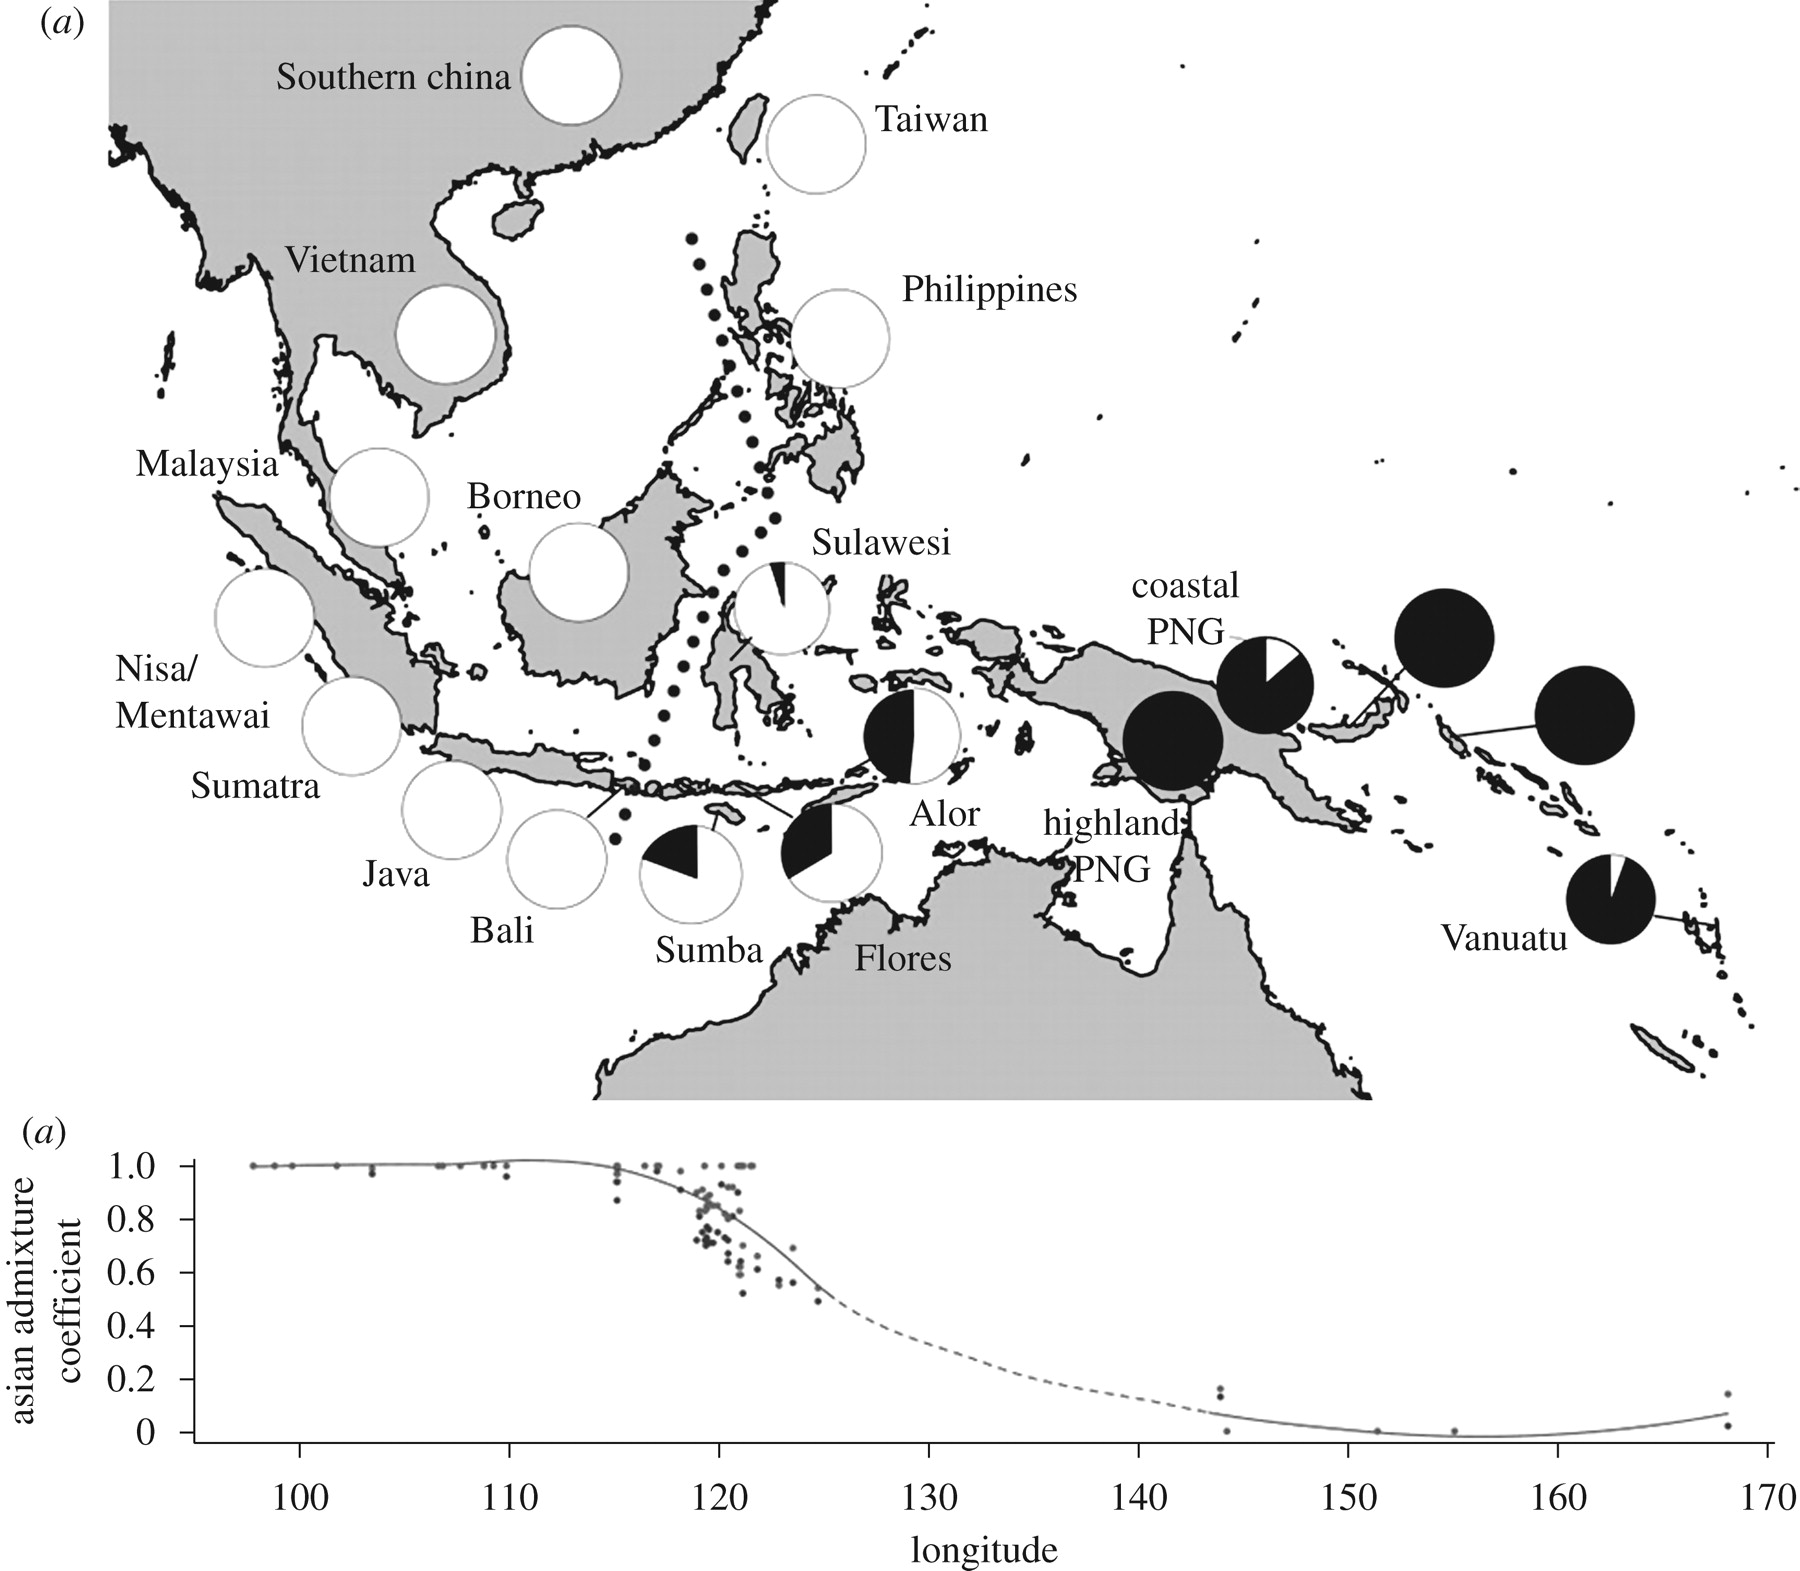
\includegraphics[width=1\textwidth]{../data/cox-image.jpg}
	\caption{Local admixture rates across the Indo-Pacific region. (a) Pie charts showing mean regional admixture rates (Asian component in white; Melanesian component in black). Wallace’s biogeographic line is shown as a dotted line. Regional admixture rates are shown for data reduction purposes; (b) Change in Asian admixture rates calculated from all SNPs combined (black line). Regions with no data indicated by a dashed line (exact gradient unknown). Asian admixture estimated from autosomal and X-chromosomal SNPs are indicated by black and grey points, respectively. Note the decline in Asian admixture beginning in eastern Indonesia, as well as preferential retention of X-chromosomal (grey) versus autosomal (black) diversity. Reproduced unmodified from \cite{Cox01}.}
	\label{cox-image}
\end{figure}

\begin{figure}[H]
	\centering
	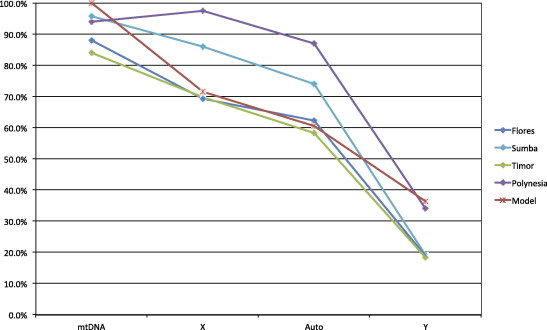
\includegraphics{../data/lansing-image.jpg}
	\caption{Fraction of Asian DNA in four genetic systems compared with model results for $\alpha = 0.02$ and 50 generations. Sample sizes: Flores = 453, Sumba = 639, Timor = 529. Reproduced unmodified from \cite{Lan01}.}
	\label{lansing-image}
\end{figure}

The whole idea of the project is thus to try to reproduce the same patterns and to determine which sets of parameters lead to outputs similar to what is observed.
The model is set to run from the beginning of the Austronesian expansion, around 4,500 years ago, to the present.

The simulated data from the model will be the observed \gls{admixture} rates of the populations in the area covered by the model.
The \gls{admixture} will be measured for five parts of the DNA: the whole DNA, the mitochondrial DNA, the autosomal DNA and the X and Y-chromosomal DNAs.
These \gls{admixture} values will only be recorded for the last step of the simulation, since they will be the only values comparable to the real observed \gls{admixture} results.

\chapter{Existing context}
\section{Agent-Based Model}
The model is an Agent-Based Model (ABM) that comprises a graph of nodes, each node corresponding to a \gls{deme}, and each edge corresponding to a possible migration route between \glspl{deme} (see Figure \ref{nodesOnMap}).
The agents of the model are people living in the graph, in every node, and these agents are able to migrate and to create families.
The graph and the agents living in it respond to a set of basic rules regulated by parameters and the goal is then to observe the emerging behaviours arising from it.

\begin{figure}[H]
	\centering
	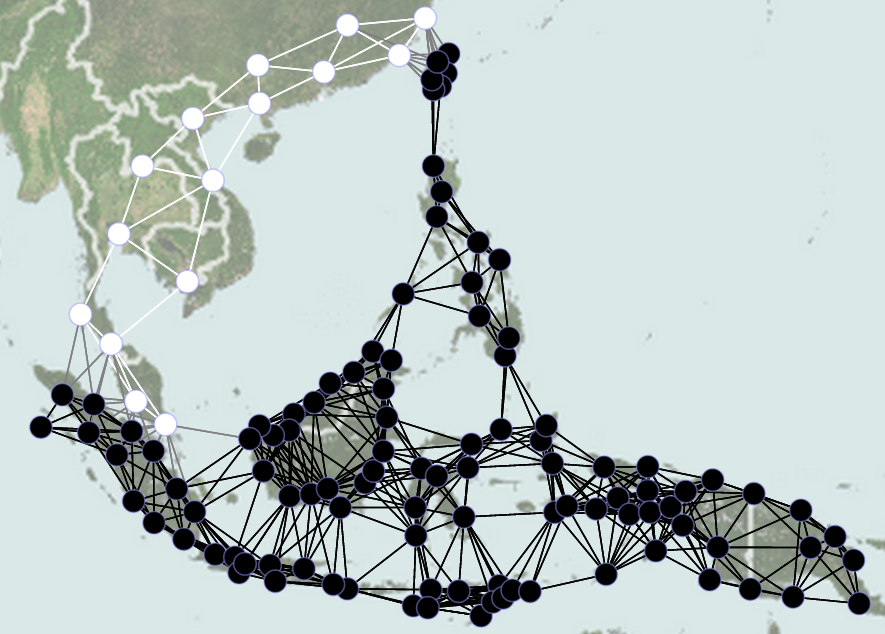
\includegraphics[width=1\textwidth]{../data/ISEA-node-map.png}
	\caption{Nodes of a model superimposed onto the map of the modelled region. White nodes are the Asian nodes at the beginning of the simulation and black nodes are the Melanesian ones, according to one of the possible starting distributions.}
	\label{nodesOnMap}
\end{figure}

Because of the stochasticity of the model, and because the parameters used might not be viable, a simulation can end up having non-usable outputs.
For example, if an island ends up being completely empty, the \gls{admixture} values yielded by this specific simulation will be the value \texttt{NaN} (not a number).
In such extreme cases, the model can be considered as “failed” and can either be discarded or given the worst possible score, depending on the current analysis.
Arbitrarily, two rules have been set to define that a simulation has failed:
\begin{itemize}
	\item If a \gls{deme} has a population of less than 10\% of the most populous \gls{deme} in the network, it is considered as empty;
	\item If more than 25\% of the \glspl{deme} in any of the islands are empty, the simulation is considered as failed.
\end{itemize}

The model itself has been developed in Java using the Repast Simphony framework (\cite{Nor01}), a cross-platform framework made to write flexible agent-based models.
The agents correspond either to a single person or a couple that evolve in the \glspl{deme}.
Each \gls{deme} is a node in the graph and possible migration paths between \glspl{deme} are edges of this graph.
Therefore, the implementation of the model consists of agents evolving in a graph.

\subsection{Parameters}
Numerous parameters can be set in the model.
Some of them are defined initially and the fact that they are immutable is to simplify the model by limiting the number of parameters to set.

The parameters that can actually be adjusted are listed in Table \ref{parameters} and can be put into different groups.
Most of them are continuous parameters, whose values are numbers, and a few of them are discrete.
The discrete parameters are the graphs used and the starting distributions.
While the former corresponds to the topology of the graph used in the simulations, comprising the nodes and the edges between them, the latter is the distribution of the Melanesian and Asian populations in the graph at the initial step of a simulation.

The model can work with a large number of different parameter values, corresponding to the “values” columns in Table \ref{parameters}.
Knowing the context of the model, especially using previous anthropological studies, an estimation of possible realistic values can be found, but will need to be refined later on during the analysis processes.

\begin{table}[H]
	\hspace*{-2.25cm}
	\begin{tabular}{|c|l|l|l|}
		\hline
 		Parameter & Values & Estimated & Comment \\ \hline
        Migration prob. & $\mathbb{R}_{0 \leq x \leq 1}$ & $\mathbb{R}_{0 < x \leq 1}$ & prob. to start migrating for a Melanesian agent \\ \hline
        Migration prob. ratio & $\mathbb{R}_{\geq 0}$ & $\mathbb{R}_{1 \leq x \leq 4}$ & corresponding ratio for an Asian agent \\ \hline
        Fecundity & $\mathbb{R}_{\geq 0}$ & $\mathbb{R}_{2.5 < x < 8}$ & Poisson law mean for a Melanesian agent \\ \hline
        Fecundity ratio & $\mathbb{R}_{\geq 0}$ & $\mathbb{R}_{1 \leq x \leq 2}$ & corresponding ratio for an Asian agent \\ \hline
        Marriage threshold & $\mathbb{R}_{-0.25 \leq x \leq 0.25}$ & $\mathbb{R}_{0 \leq x \leq 0.25}$ & affects marriages rules \\ \hline
        Growth rate & $\mathbb{R}_{0 \leq x \leq 1}$ & $\mathbb{R}_{0 < x < 0.001}$ & limiting rate of pop. growth \\ \hline
        Number of agents & $\mathbb{Z}_{\geq 0}$ & $\mathbb{Z}_{100 \leq x < 400}$ & pop. size in each \gls{deme}, initially \\ \hline
        Graph & \{...\} & \{...\} & composition of the graph (nodes and edges) \\ \hline
        Starting distribution & \{...\} & \{...\} & distribution of pop. in the graph \\ \hline
        % Model rules & \{...\} & \{...\} & different model rules, mainly marriages rules \\ \hline
	\end{tabular}
	\caption{Summary of the changeable model parameters.}
	\label{parameters}
\end{table}

\subsection{Other existing models}
This model is just one of the types of models that could have been chosen.
For example, other models can have their time unit defined as a generation (roughly equivalent to 20 years).
Here, the unit of time has been defined as one year to have more precise time steps in the model and to be closer to reality due to the higher time resolution.

Coalescent models also exist.
They take the problem the other way around by trying to rebuild the past, the ancestry of the individuals, based on the present data.
They do it this way to try to reduce the amount of computation needed, as they therefore do not have to simulate agents whose lineage would have ended up extinct.
It is not suited for this agent-based model though because parameters vary among agents and this is not trivial to do with coalescence.
The fact that an agent has either a Melanesian or Asian ancestry leads to different behaviour and this is more straightforward to do in an ABM.

\section{Statistical analysis framework}
Because of the complexity of the model (number of agents, stochasticity, multiple parameters), it will need to be run thousands of times and with a lot of different changing values for the parameters.
This will lead to the use of a robust statistical analysis frameworks to extract meaningful information from the high quantity of generated data.

\subsection{Comparisons}
\label{subsection:comparisons}
To compare two different scenarios, comparison functions had to be defined.
These functions will be able to provide a value of similarity or dissimilarity when provided with observable values that characterise the scenarios.
In this case, the comparison is done between the real observed data and the output of one simulation.
Every simulation output has to be treated in the same way than the observed data.
Doing so allows them to be compared.
The observed data does not include values for specific islands even though they are included in the simulations (see Table \ref{islands}).
This is because nodes had to be placed in the model so that the agents could migrate, even though the empirical studies did not get samples from the corresponding areas.
The \gls{admixture} values for mitochondrion and Y-chromosome are also not available for every island.
Those values in the model outputs can thus be dropped as they cannot be compared.

\begin{table}[H]
	\centering
	\begin{tabular}{|l|c|c||l|c|c|}
		\hline
 	  Island & Simulated & Observed & Island & Simulated & Observed \\ \hline
    Alor & \checkmark & \checkmark & Philippines & \checkmark & \checkmark \\ \hline
    Aru & \checkmark &  & Seram & \checkmark & \\ \hline
    Bali & \checkmark & \checkmark & Sulawesi & \checkmark & \checkmark \\ \hline
    Borneo & \checkmark & \checkmark & Sumatra & \checkmark & \checkmark \\ \hline
    Bougainville &  & \checkmark & Sumba & \checkmark & \checkmark \\ \hline
    China & \checkmark & \checkmark & Taiwan & \checkmark & \checkmark \\ \hline
    Flores & \checkmark & \checkmark & Tanimbar & \checkmark &  \\ \hline
    Halmahera & \checkmark & \checkmark & Thailand & \checkmark &  \\ \hline
    Java & \checkmark & \checkmark & Timor & \checkmark & \checkmark \\ \hline
    Laos & \checkmark &  & Vanuatu &  & \checkmark \\ \hline
    Malaysia & \checkmark & \checkmark & Vietnam & \checkmark & \checkmark \\ \hline
    New Guinea & \checkmark & \checkmark &  &  & \\ \hline
	\end{tabular}
	\caption{List of islands (or areas) in the model and in the reference data.}
	\label{islands}
\end{table}

The first, and most straightforward way to compare the two sets of data was to do a pairwise distance between real and simulated values.
But doing so would mean dropping a lot of information, mainly regarding the relative geographical position of every island in the region.
Another measure was needed that would keep this information and take it into account while comparing the data.
Also, the idea arose to compare the whole matrix of differences in \gls{admixture} among islands instead of the values island by island.

Sixteen comparison functions were tested with randomly generated data.
Seven were distances, including weighted versions of the comparisons.
Nine were correlation measurements, and different correlation coefficients were tested.

These randomly generated data had the same structure as the simulated data that would be later compared but the actual values, while still being \gls{admixture} values (a proportion value between zero and one), were completely random.
When comparing the results of the comparison functions with the same random data, functions that would yield correlated results would convey the same information.
It would thus make no sense to choose two functions whose results are highly correlated because it would mean adding dimensions to the comparison values while not adding any meaningful information.

Two measures have been selected that can hold different information about a comparison: the mean square distance (MSD) and the partial Mantel test.
They do not have a good correlation when applying them to random \gls{admixture} values, thus meaning that they do not carry the same information.
They are complementary, and using them both gives a better overview of the comparison.

\subsubsection{Mean square distance}
The mean square distance is the mean value of all of the distances between observed and simulated values of \gls{admixture} for every $n$ island.

\begin{equation}
MSD = \frac{\sum\limits_{i=1}^{n} (AdReal_i - AdSim_i) ^ 2}{n}
\end{equation}
where $AdReal$ is the array of \gls{admixture} data observed in the real values and $AdSim$ the corresponding values in the simulated model.

It gives a distance value, with zero meaning that the two observed values are absolutely identical.
In this specific context, taking into account that the compared values are \gls{admixture} values, ranging from zero to one, and because of the values observed in the real data, the highest possible MSD value will be around $0.8$ (see reference case lines in the upper part of Figure \ref{app:sensit-comp-1d}).


\subsubsection{Partial Mantel test}
The Mantel tests have been developed to compare two matrices with the same information.
The partial Mantel test also uses a third matrix, holding constant geographical distances in order to be able to weight the values according to the actual geographical distances between the points (\cite{Smo01}).

In this case, the first two matrices contain the values of distances in \gls{admixture} between every island in the graph and a matrix $M$ is calculated as
\begin{equation}
	M = \begin{bmatrix}
		d(Ad_0, Ad_0)	& \cdots & d(Ad_0, Ad_n) \\
		\vdots			& \ddots & \vdots		 \\
		d(Ad_n, Ad_0)	& \cdots & d(Ad_n, Ad_n)
	\end{bmatrix}
\end{equation}
where $d$ is the function returning the distance between the two arguments and $Ad_{n}$ is the \gls{admixture} of the $n$\textsuperscript{th} island in the graph.
With the corresponding matrices for the simulated data, the real data and also the geographical distances, the partial Mantel test can be done as such
\begin{equation}
	correlation = partial.Mantel(M_{Simulated}, M_{Real}, M_{geographical})
\end{equation}

The partial Mantel test returns a correlation value between -1 and 1 with a value of 0 meaning that the two matrices are not correlated at all and 1 if they are completely correlated.


\subsection{Approximate Bayesian Computation}
A fairly recent statistical analysis framework has been used more and more in the context of population simulations.
This framework is called Approximate Bayesian Computation (ABC).
Its use is recommended when using high dimensional data that makes it difficult to use standard statistical frameworks.
ABC still relies highly on standard statistical tools but instead of giving one best result, it returns a distribution of best possible parameters.
It answers the question: given a set of parameter distributions (called “\glspl{prior}”), what are the distributions (subsets of the \glspl{prior}), that give best results? This set of output distributions are then called “\glspl{posterior}”.

Its use has been increasing recently and some examples of recent papers using ABC in similar contexts are \cite{Gui01} or \cite{Keh01}.

The whole framework encompasses the steps from the choice of the parameter sets to the inference of the posterior distributions.
Figure \ref{abc} summarises the successive steps of this process with hypothetical parameters $\alpha$, $\beta$ and $\gamma$ and summary statistics $SS1$ and $SS2$.
The parameters will be used by the model to generate results.
These results are, either directly or after transformation, the summary statistics that the ABC will use.
By comparing those to the references, the framework is able to keep or discard a simulation during what is called the rejection step.
the parameters whose simulations got accepted can be used and visualised in distributions.

\begin{figure}[H]
	\centering
	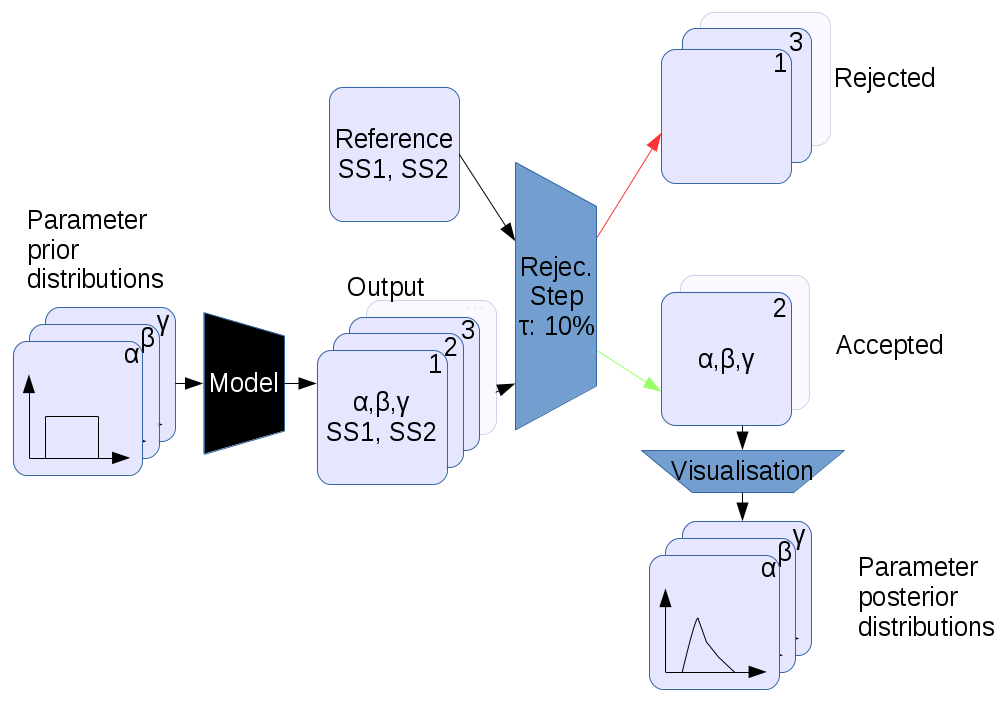
\includegraphics[width=1\textwidth]{../data/abc-landscape.png}
	\caption{Visual representation of the different steps of an ABC inference framework.}
	\label{abc}
\end{figure}

The \glspl{prior} are defined as a set of distributions, one for each observed parameter.
The distributions can be of any type but it is necessary to know them when doing the inference of the \gls{posterior} distributions since, depending on the type chosen, they can induce a bias that will need to be corrected.
In general, for ABCs, uniform, Poisson or normal distributions are used.
Here, the distributions chosen are all uniform and the only bias can be if the correct parameters lay outside of the boundaries of the distributions (thus the importance of the previous grid search analysis).
A visualisation of example simulation parameter sets that can be generated by the first step of an ABC framework can be seen in Figure \ref{abc-space}.

\begin{figure}[H]
	\centering
	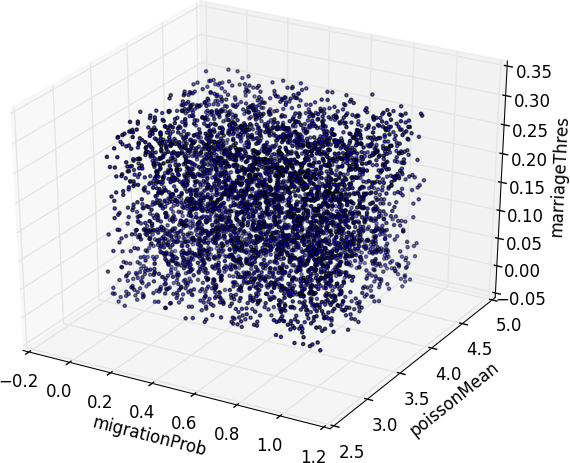
\includegraphics[width=0.8\textwidth]{../data/abc-space.png}
	\caption{Visual representation of 5,000 sets of three parameters, $migrationProb$, $poissonMean$ and $marriageThres$ drawn from independent uniform distributions. As a result, the points are evenly spread inside a cuboid. Each point represents one set of parameters that will be used for one single simulation.}
	\label{abc-space}
\end{figure}

Now that the required parts are defined, their implementation is needed, taking into account the specifics of the project.


\chapter{Implementation}
The different parts of the statistical analysis pipeline implementation are detailed in the next sections.
A global overview of the pipeline is available in Figure \ref{workflow-2} and presents the different modules of the pipeline, the language in which they were written, as well as the formats of the intermediary storage steps.
The modular design is necessary because the analysis pipeline requires high flexibility.
The arrows in Figure \ref{workflow-2} only represent a few of the possible ways the pipeline can be used, and depending on what is necessary, some intermediary steps can be bypassed.
Also, with the same idea of flexibility and ease of use, every script can be called independently and provides command line parameters defined in a standard way (POSIX\footnote{Portable Operating System Interface} guidelines) and a corresponding help option to detail them.

The model here has been simplified to a single step in the pipeline even though it is fairly complex.
This is because the implementation of the model, while it is really important for the project, does not enter in the scope of the internship.
Its inner functioning and design is nevertheless required for the implementation of the rest of the pipeline.

\begin{figure}[H]
	\centering
	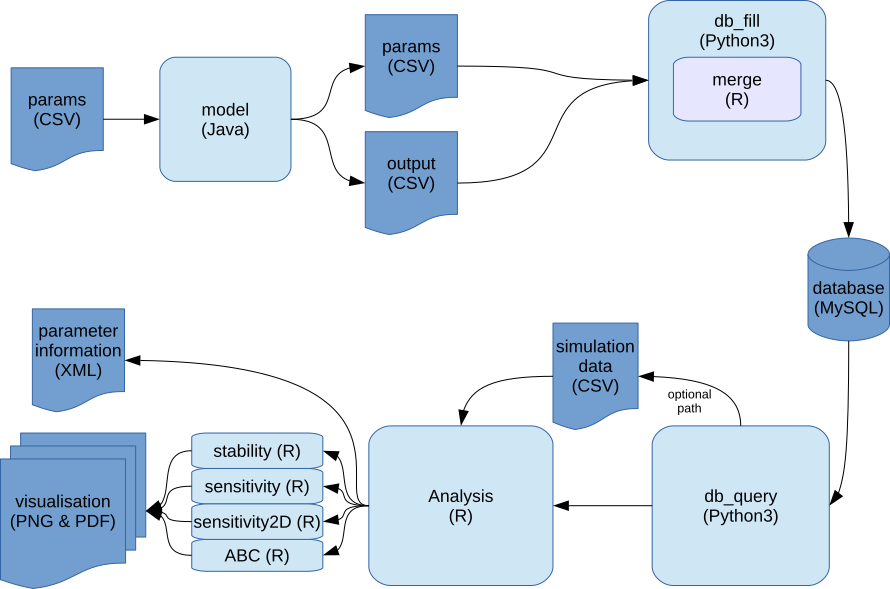
\includegraphics[width=1\textwidth]{../data/workflow-2.png}
	\caption{Visual representation of the different parts of the treatment and analysis pipeline. Dark colours represents data and the way it is stored, and light colours represent programs and scripts and the language in which they have been written.}
	\label{workflow-2}
\end{figure}



\section{Run management}
The fact that many simulations are required to infer meaningful information from the model implies that they cannot be run sequentially on a single desktop computer in a reasonable amount of time.
Luckily, every simulation being independent from the others, there are multiple ways to generate more results in less time.
Firstly, if the computer used has multiple processors, it can run multiple simulation concurrently.
Also, a cluster of computers can be used and the simulations needed can be dispatched among the nodes of the cluster so that they each run the simulations they were assigned.
When all of the nodes have ended their runs, their outputs can be aggregated and/or stored.

Different levels have been used.
First, running the simulations locally (Figure \ref{network:local}), on a single computer, then using the three computers in the office as a cluster of compute nodes (Figure \ref{network:office}), for more heavy batches.
Also, since Massey University just made an agreement with Microsoft Azure, which provides computing “in the cloud”, simulations have been run transparently by adding virtual machines on the Microsoft Azure system to the cluster of computers in the office (Figure \ref{network:azure}).
Finally, when the computation requirements were too high, for really huge batches, NeSI\footnote{New Zealand eScience Infrastructure: \url{https://www.nesi.org.nz/}}’s High Performance Computing (HPC) facilities have been used (Figure \ref{network:nesi}).
They provide servers specially designed for scientific computation and can be tasked with hundreds of parallel jobs at a time and multiple batches can be queued so they will be run as soon as computational power is available.
Each node is an IBM Power755 machine.

The most powerful level used for this study is obviously the HPC but a trade-off of using this system is that, since it is shared by multiple users and is managed by a third-party, it requires specific settings and it cannot be used exactly as can a custom cluster of computers.
The batches have to be submitted through a \gls{job-scheduler}, in this case called LoadLeveler.
Because of this, slight changes have been made to the way the model and the Repast framework are launched.
Simulations run on this HPC use several nodes, with each of these nodes having multiple threads available for the simulations.
This configuration leads to the parallel simulation of more than a hundred scenarios at the same time.
In this case 4 nodes were used, each of those having 32 threads.

\begin{figure}[H]
	\centering
	\begin{subfigure}[t]{0.4\textwidth}
		\centering
		
\includegraphics[scale=0.5]{../data/network:local.png}
		\caption{local}
		\label{network:local}
	\end{subfigure}
	~
	\begin{subfigure}[t]{0.4\textwidth}
		\centering
		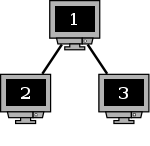
\includegraphics[scale=0.5]{../data/network:office.png}
		\caption{local network}
		\label{network:office}
	\end{subfigure}
	\\
	\begin{subfigure}[t]{0.4\textwidth}
		\centering
		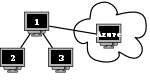
\includegraphics[scale=0.8]{../data/network:azure.png}
		\caption{local network and Azure}
		\label{network:azure}
	\end{subfigure}
	~
	\begin{subfigure}[t]{0.4\textwidth}
		\centering
		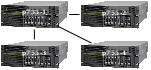
\includegraphics[scale=0.8]{../data/network:nesi.png}
		\caption{NeSI}
		\label{network:nesi}
	\end{subfigure}
	\caption{Different set-ups to run the model.}
	\label{network}
\end{figure}

\section{Data processing, storage and querying}
Since running a lot of simulations, with a lot of different parameters, can generate a lot of output files whose original parameters can be hard to track, a way to keep them organised was needed.
Doing so, it would also be possible to use results from different batches and to analyse them together, thus avoiding having to redo simulations for parameter values already tested and reducing the computation resources used.

The organised way to store this is naturally in a database.
The choice has been made to use a relational database.
The structure and indices have been designed so that the parameters can be efficiently queried.
The tables and relations between them can be seen in Figure \ref{db}.
It has first been developed and tested locally and then, once it was working properly, it was deployed on a MySQL database server provided by Massey University for research purposes.

\begin{figure}[H]
	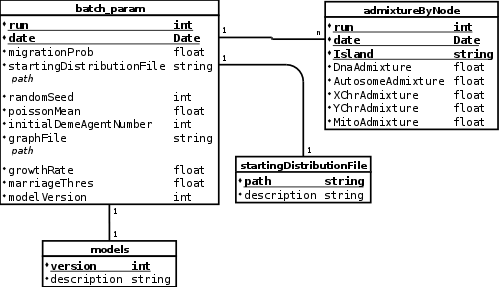
\includegraphics[width=1\textwidth]{../data/DB.png}
	\caption{Structure of the database storing the results of the simulations and the corresponding parameters.}
	\label{db}
\end{figure}

The use of the database can be done through phpMyAdmin but two scripts have been developed to interact with it directly.
The first one reads the two files output by the model (the \gls{admixture} data and the corresponding parameter values), merges them and adds the resulting data to the database.
The other one queries the database according to conditions provided by the analyst and returns already merged parameter and admixture values.
The scripts have been written in Python3, using the PyMySQL module to access the MySQL database.
Internally, the first script to add data to the database uses another script, in R, that processes the data before adding them.
This way one process, the Python script, handles the connection with the database while another process, the R script, does the actual data processing at the same time, in parallel.

\section{Statistical analyses}
\subsubsection{Grid search}
In order to reduce the parameter space, a grid search has been performed.
It consists of going through the possible parameter sets by setting parameter values at regular steps throughout the space and running $n$ multiple simulations for every point in the space to obtain statistically meaningful results for every point.
One parameter grid search can be seen in Figure \ref{grid}.

\begin{figure}[H]
	\centering
	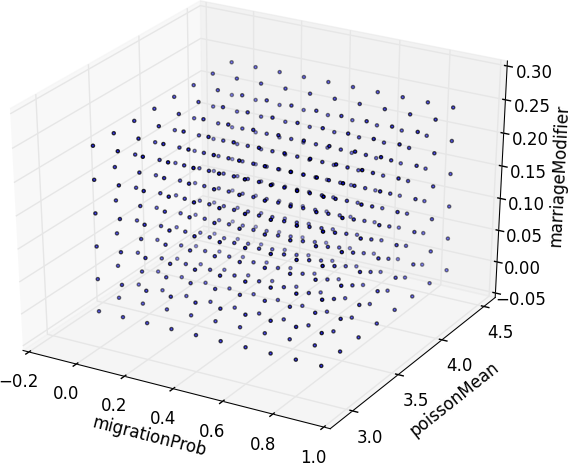
\includegraphics[width=0.8\textwidth]{../data/grid.png}
	\caption{Visual representation of a grid search on three parameters, $migrationProb$, $poissonMean$ and $marriageThres$. Each point represents a set of those parameters, that will be used for $n$ different simulations.}
	\label{grid}
\end{figure}

Depending on the number of parameters and the step sizes, this has an important computational cost.
This has been considered a necessary step though, in order to reduce the parameter space for the next analysis, the ABC analysis, that would be even more computationally consuming if run over a huge parameter space.
The resulting parameter space that will be used after the grid search analysis is defined manually after selecting interesting and meaningful values that can either be a smaller space or a specific value, thus making a parameter a non-changing one. Details of this will be presented in Section \ref{section:results:grid}.

\subsubsection{ABC framework}
Once an interesting subspace of parameters has been defined, it can be used to feed the ABC framework used later.
Whereas a standard Bayesian analysis can be used to infer a single best value for every parameter, here the use of ABC gives a posterior distribution of parameters corresponding to the best values.
The shape of the distributions can thus be appreciated and this offer better understanding of the output values of highly stochastic models run a large number of times.
This technique, although quite recent, has been described in numerous studies (\cite{Sun01, Csi02}).

In this project, the parameters used are the ones defined in Table \ref{parameters} even though the ones set after the grid search analyses will be ignored by the ABC as they are defined once and will not change.
They are simply not defined by a distribution as they are constant, and running them through the ABC is useless.
The summary statistics will be the four results of the comparison functions defined in section \ref{subsection:comparisons}: the MSD and the partial correlation for both the X-chromosome and the autosomes.

At first, the R package “abc” \cite{Csi01} was used to understand how it worked and to be sure that the framework was used correctly.
But in the end, to simplify the pipeline and to cope with the specifics of the project, custom code inspired by the R package was written.
The main difference is that, instead of using the results of the comparison functions as summary statistics that would be fed into the package, these results are directly used to accept or reject a simulation.
Also, changes have been done so that the ABC analysis fits better into the project and provides more useful information for this use case.
For example, since the change to custom code there is no need to reshape the R data to run the rejection step, and the threshold for this step is also easier to change without rerunning the whole analysis.

The first step of the ABC consists of generating the \glspl{prior}.
This is done via a custom Python3 script which uses a parameter file (YAML format) into which the distributions are defined.
The script generates $n$ parameter sets that will be used as is by the model.
The randomness of the generated values among the distributions is very important for the \gls{posterior} inference so this aspect has been taken into account, otherwise the results could become biased.

After the model has generated results for every parameter set, the ABC framework needs to choose which simulations are closest to the reference data.
In this case a rejection step with a tolerance has been implemented.
For a tolerance $\tau=10\%$ for example, the ABC will keep the $10\%$ of the simulations whose results are closest to the reference.
It is important to have a low tolerance taking into account that most of the parameter space is expected to give “bad” results.
The tolerance can be adjusted for every analysis and no perfect tolerance exists; this instead has to be defined by the analyst using the ABC.

Finally, the parameter values for the selected simulations are retrieved and the corresponding distributions form the \glspl{posterior}.
These inferred distributions are the actual result of the ABC and can be used to deduce which parameter values, and which ranges, are more likely to yield results close to the observed reality.

\section{Visualisations}
As said in \cite{Wei01}, it is easy to represent data but hard to represent it so that the person visualising it does not need to dig into the huge quantity of data again to understand what is happening.
It is important to represent the data well so that it is useful to the analyst.
A trade-off has been found between showing as much data as possible and doing visualisations easy to understand and showing what it is expected from a specific type of visualisation.

For this, an important part was to try to avoid simplistic visualisations when they would not show enough information.
For example, a simple mean or median value is not enough when there are alternative ways to represent these data.
Whenever possible, notched box-plots were used to show the distributions and shapes of the data.
The box-plot centre of the box-plot represents the median, the interquartile range is represented by the box and outside of the whiskers are possible outliers from the data.

In some cases, too many box-plots would overwhelm the analyst so, as an alternative, mean values are used but with additional error bars corresponding to the standard deviation in order to quickly evaluate the significance of the differences between the displayed values.

To let the viewer easily grasp diverse data, even though the values are different and work differently, they share a single colour theme.
For example, low distance values and high correlation values are both displayed in green colours, as a way to signal “good” values.
Inversely, high distances and low or opposite correlations are displayed in red shades as a way to show that they represent “bad” values in the specific context of this project.

Figure \ref{preview-heatmap} shows a part of an example visualisation showing with good and bad correlation values for the autosomal and X-chromosomal admixtures.
Low correlations appear in specifics areas of the parameter spaces where both the migration rates ($migrationProb$) and the fecundity ($poissonMean$) are either low or high.
A strip of high correlations is visible and reveals a trade-off between these two parameters.

\begin{figure}[H]
	\centering
	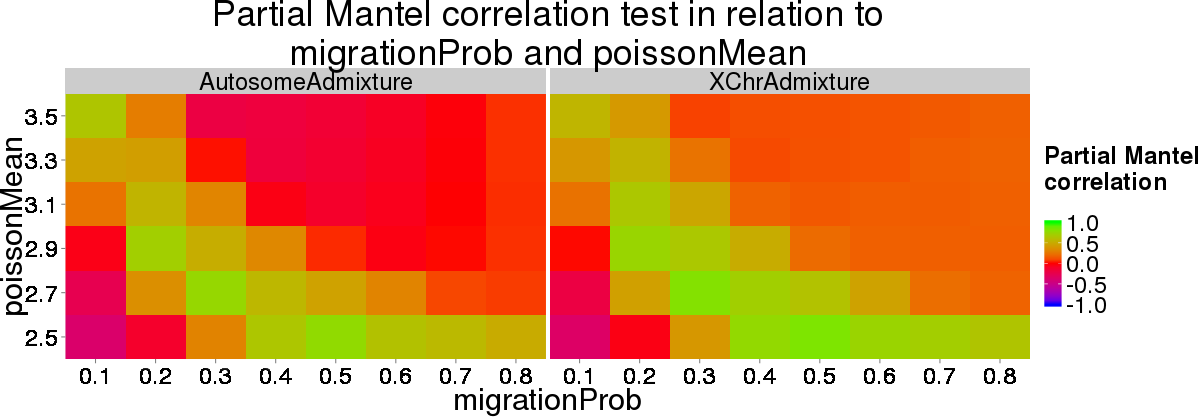
\includegraphics[width=1\textwidth]{../data/sensit-comp-2d-preview.png}
	\caption{View of a part of an output graph, highlighting the different possible colours in the visualisation. The complete graph is in the appendices, Figure \ref{app:sensit-comp-2d}.}
	\label{preview-heatmap}
\end{figure}

Examples are available in the appendix (see section \ref{app:ex-visu}) and are made in R using the ggplot2 library \cite{Wic01} to get nice looking graphs while having simpler and thus more maintainable code.
They will be detailed while presenting the results in chapter \ref{chapter:results}.

Also, a common theme has been defined for all the visualisations to have consistent colours, fonts, and sizes among the different generated images.
Finally, the images are saved in a raster format (PNG) but also in a vector format (PDF).
Because of this vectorial output, changes can be applied to the images for publication, for example if a specific aspect ratio is required or if changes need to be made to the positioning of legends or scales.
More importantly, this is the only way to have a lossless format that can be resized without quality loss.

\subsubsection{Other visualisations}
The visualisations were made and adapted on the fly so that they could be used to help make decisions and choices.
They can still change and be adapted to new needs and that is supposed to be made easier through the use of adapted R libraries like ggplot2 that add a layer of abstraction above standard R code.
The code responsible for the visualisations is also restricted to specific parts of the pipeline, making it highly modular and easy to change or to replace.

Until now, the graphs generated were limited to two-dimensional graphs, mainly for easier understanding and integration in papers, but one way to add more information can be through the use of three-dimensional graphs or animated graphs so that a higher number of model parameters can be visualised at the same time.
It is important though that those new visualisations keep a certain level of readability that can easily be lost with higher dimensional graphs.


\section{Optimisations}

\subsubsection{Computational cost}
Some key steps in the analysis framework need to be efficient enough so that time is not lost waiting for results to be treated or for graphs to be plotted and that the computation can be done without needing a supercomputer.
This project has seen a few important refactoring steps to be able to cope with the quantity of data to be treated.
The most important one has been to start treating the simulation results as a stream of values instead of loading the whole dataset in memory.
This was the only way to make the whole analysis process really scalable and to be able to handle a very high quantity of data.

This changed the memory complexity from linear to constant and it actually improved the time complexity from sub-quadratic to linear for the treatment part and from sub-quadratic to linearithmic ($n$ log $n$) for the analysis part.
The improvement in time has been made possible by assuming that the results of one simulation are always together in the result stream, that way saving the cost of searching results in a big block of memory when they are actually next to each other.
Actual execution times have been recorded and can be seen in appendix \ref{app:bench} in graphs \ref{app:bench-merging-time} for the treatment step and \ref{app:bench-analysis-time} for the analysis step.
The corresponding maximum memory use values are shown in the graphs \ref{app:bench-merging-mem} and \ref{app:bench-analysis-mem}.

There is effectively still a great amount of room to improve memory usage, especially seeing that the base memory usage is between 60 and 200 MB just when loading libraries, functions, global variables and set-up code.

The stream approach also allows the different steps of an analysis to be run simultaneously, by piping each step to the next, effectively making the whole process able to be in parallel.
This is useful only if the computer used has at least $n$ cores if $n$ processes need to be run in parallel.
In this case, the time of the whole process is the time needed to run the longest step.

\subsubsection{Importance of randomness}
One important aspect that has been discovered while working with the Repast framework is the way it handles randomness.
For a stochastic simulation, randomness is key, since starting two simulations with the same random seed and the same parameters would lead to the same succession of events in the simulation and thus to the same outcome.
These two simulations would actually be identical.

When looking at the results from a statistical point of view, two identical simulations cannot be used as two distinct values.
This would simply make no sense and lead to biased interpretations of the values.

The problem with Repast is that it uses the current time to generate a random seed.
This can be acceptable when the program is run on one thread on a single computer, since the time at which one simulation starts will always be different from one simulation to another.
It might lead to problems if the simulations are run in parallel using multiple threads on the same machine and/or using different machines and they happen to start at the same time.
The risk of both the random seed and the parameter set used for the simulations colliding, while not probable, is still possible and thus not acceptable.
Actually, even though the random seed is supposed to be a 32 bit signed integer, meaning that there are more that 4 billion possibilities, collisions happened more than once during this project.

The first way to handle this has been to alert the analyst when this happened so that they could remove the specific simulations if needed.
Secondly, a way has been found to generate the random seeds for the ABC analysis beforehand using \textsc{unix}’s random source, \texttt{/dev/urandom/}, that can generate pseudo-random values which can be used for cryptographic purposes, meaning that it is good enough in this case to avoid collision.

~\\

After implementing all of this, the results can be analysed and different interpretations can start to be given.

\chapter{Statistical analysis results}
\label{chapter:results}

\section{Grid search analysis}
\label{section:results:grid}
\subsubsection{Stability analysis}
For the outputs from simulations with grid searches, multiple types of analysis were used, depending on the needs.
The first one was to look at a specific point of the grid and assess the stability of the output generated with this parameter set.

The stability analysis outputs different views of the data for this point in the grid.
The first ones are 4 graphs, one for each type of observed DNA, for which box-plots for the \gls{admixture} values of each island are displayed (partial view in Fig. \ref {preview-boxplot}, complete view in Fig. \ref{app:stability}).
The size and spread of the box-plots represent the variability of the data among the different simulations with the same input parameters.

With “correct” parameters, the \gls{admixture} values are supposed to be less stable in the contact zones between the different populations at the end of the simulation than in the extremities of the graph, where the source populations live.
In the simulations used to create Figure \ref{preview-boxplot}, the Philippines were a contact zone between the two populations after the 4,500 years simulated.
The corresponding box-plots (the fifth from the left) are indeed more spread than most of the others.

\begin{figure}[H]
	\centering
	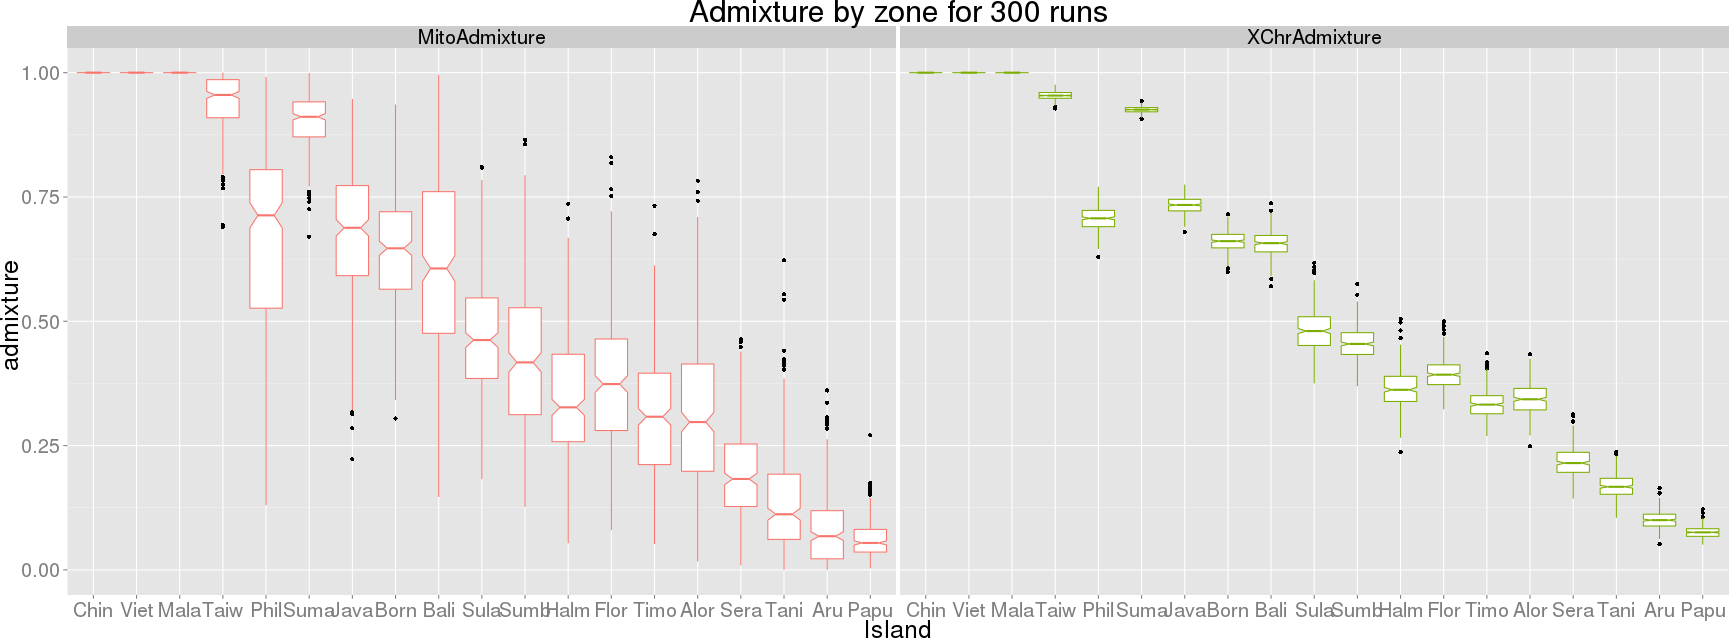
\includegraphics[width=1\textwidth]{../data/stability-preview.png}
	\caption{View of a part of an output graph, showing box-plots for mitochondrial and X-chromosomal admixture values by island. The complete figure is in the appendices, Figure \ref{app:stability}.}
	\label{preview-boxplot}
\end{figure}

Less stability is also expected when looking at \gls{admixture} values comprising fewer markers.
That is the case with mitochondrial and Y-chromosomal \gls{admixture} where the corresponding DNA only have one marker each, whereas X-chromosome and autosome have 25 makers each, leading to more stable admixtures.

And finally, lower stability is expected from islands that include fewer \glspl{deme}, and thus lower population sizes, like Alor, Aru or Bali that are composed of only one single \gls{deme} each when New Guinea (Papu in the figures) has twenty.

If the parameter value set induces abnormal behaviour, it thus means that it is not a realistic set of values.

Another view that is output by the stability analysis is the graph of \gls{admixture} values as a function of the types of DNA, and for every island (Fig. \ref{stability-admixGradient}).
This graph aims to resemble Figure \ref{lansing-image} (\cite{Lan01}) as a way to compare the real data in this paper to the data generated in the simulations.

\begin{figure}[H]
	\centering
	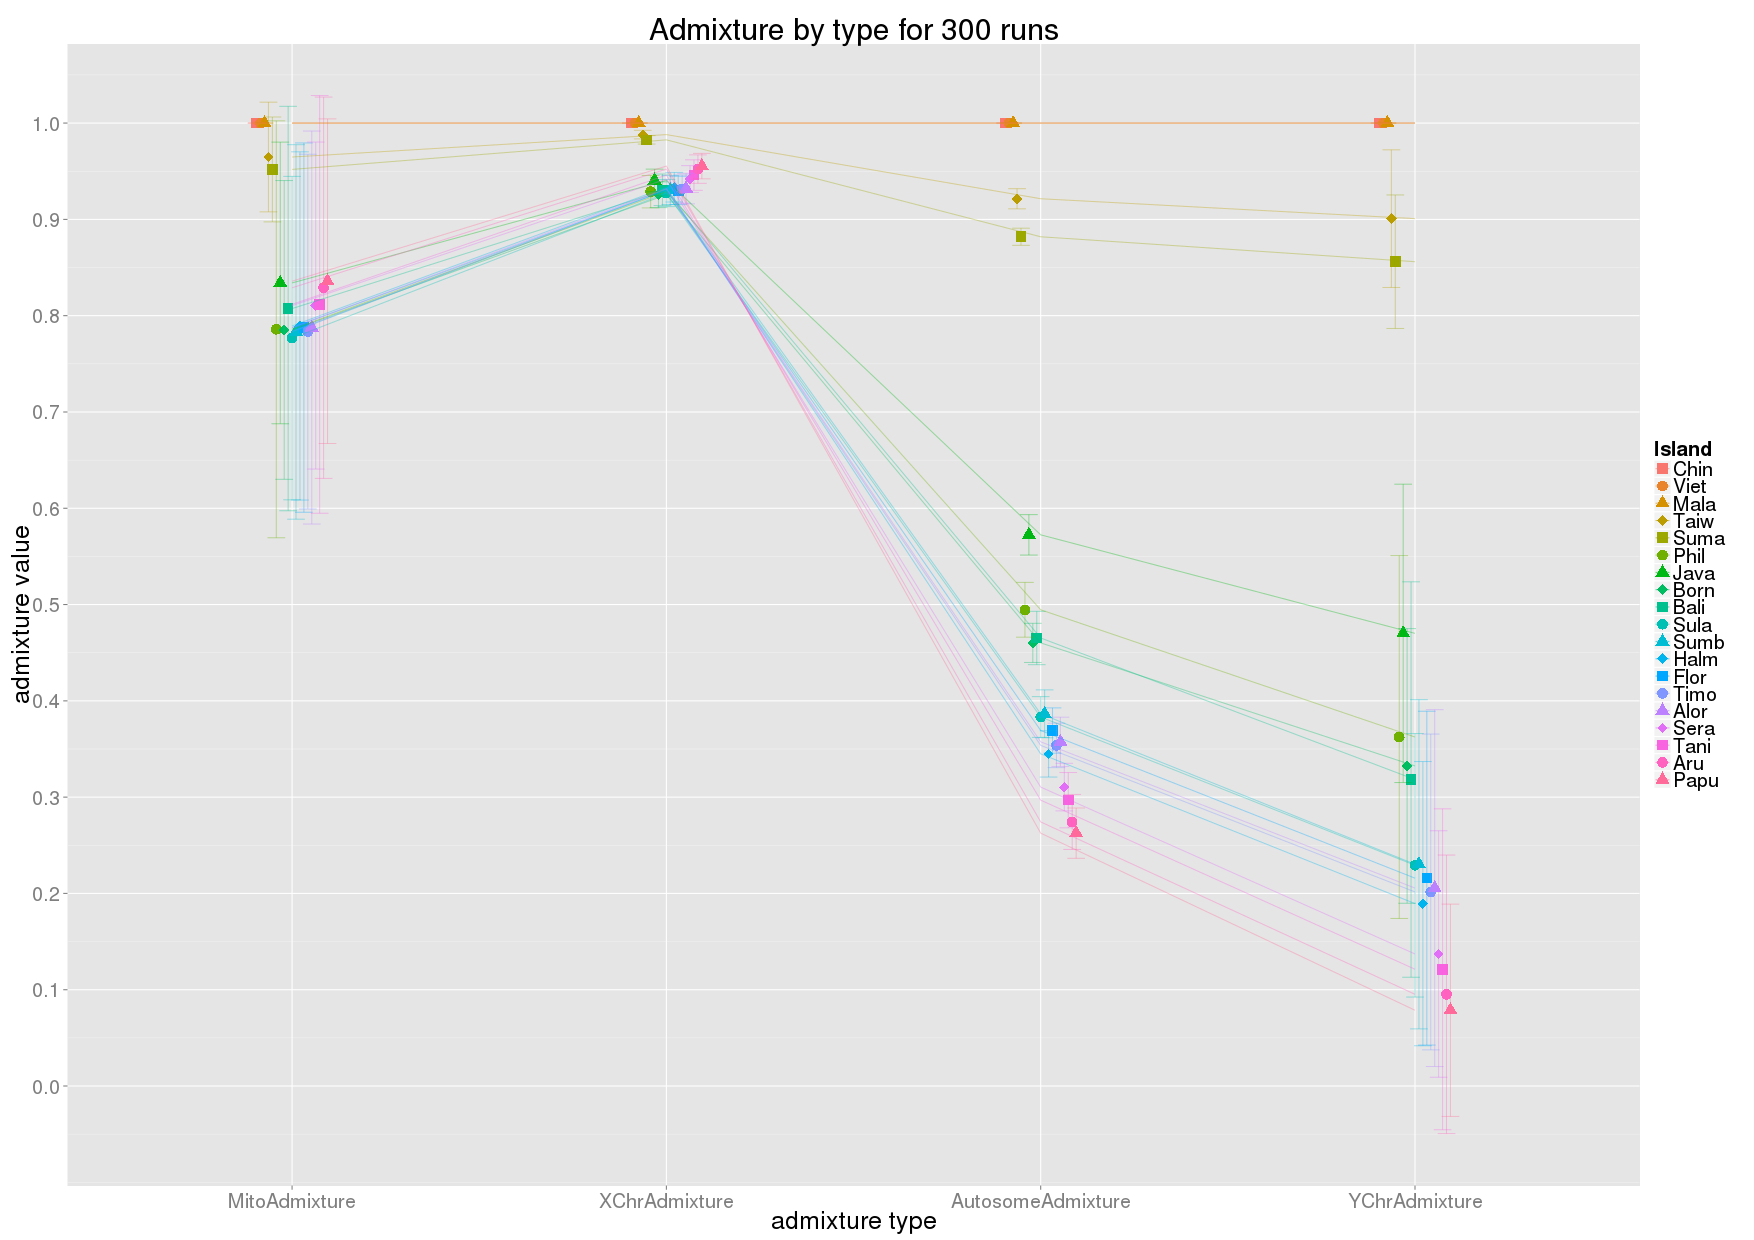
\includegraphics[width=1\textwidth]{../data/stability-admixGradient.png}
	\caption{Admixture values by type of DNA, for every island.}
	\label{stability-admixGradient}
\end{figure}

\subsubsection{Sensitivity analysis}
When looking at lines or planes on the grid, the sensitivity of the output to changes in the corresponding parameters can be analysed.

At first, this analysis was done by looking at a single changing parameter while the others were fixed at one value.
This was called a one-dimensional sweep and corresponds to parameter values aligned on a one-dimensional line in the grid.
Then this could be done on a two-dimensional sweep, corresponding to a plane.

Even though it was technically possible, no higher dimension was analysed because of the difficulty of further visualising the results.
Indeed, the visualisation choices would have needed three or higher-dimensional visualisations and those are less straightforward to represent and to analyse.
There is absolutely no limitation to the dimensionality when running the simulations, and batches were actually regularly run with more than two dimensions.
Only the visualisation has limitations with high numbers of dimensions, which is why a subset of the simulations were used when performing the visualisation.

The first thing checked is the count of simulations for every point in the grid.
This is done to be sure that, during the further steps, similar number of simulations will be compared.
Otherwise, and especially when there are low numbers of simulations, results can be biased and the standard deviations can be non-comparable.
An example of this visualisation can be seen in Figure \ref{app:count-2d}.

Then, comparisons to the real data are performed, for both the autosomal and X-chromosomal DNA data (see section \ref{subsection:comparisons}) and the resulting values are displayed so they can be analysed by the analyst as seen in Figure \ref{app:sensit-comp-1d} and \ref{app:sensit-comp-2d}.

Because of this analysis, specific values of migration have been discarded.
Really low migration ($migrationProb < 0.1$) or nearly systematic migration ($migrationProb > 0.8$) are conditions in which it gave clearly bad results.
The parameter space for the migration probability has thus been reduced to $[0.1, 0.8]$ when doing further analyses.

Also, really low fecundity rates gave too many failed simulations. Because $poissonMean$ values below $3.5$ were thus considered unrealistic, the space was reduced to only include values higher than $3.5$.

\section{ABC framework}

\begin{figure}[H]
	\centering
	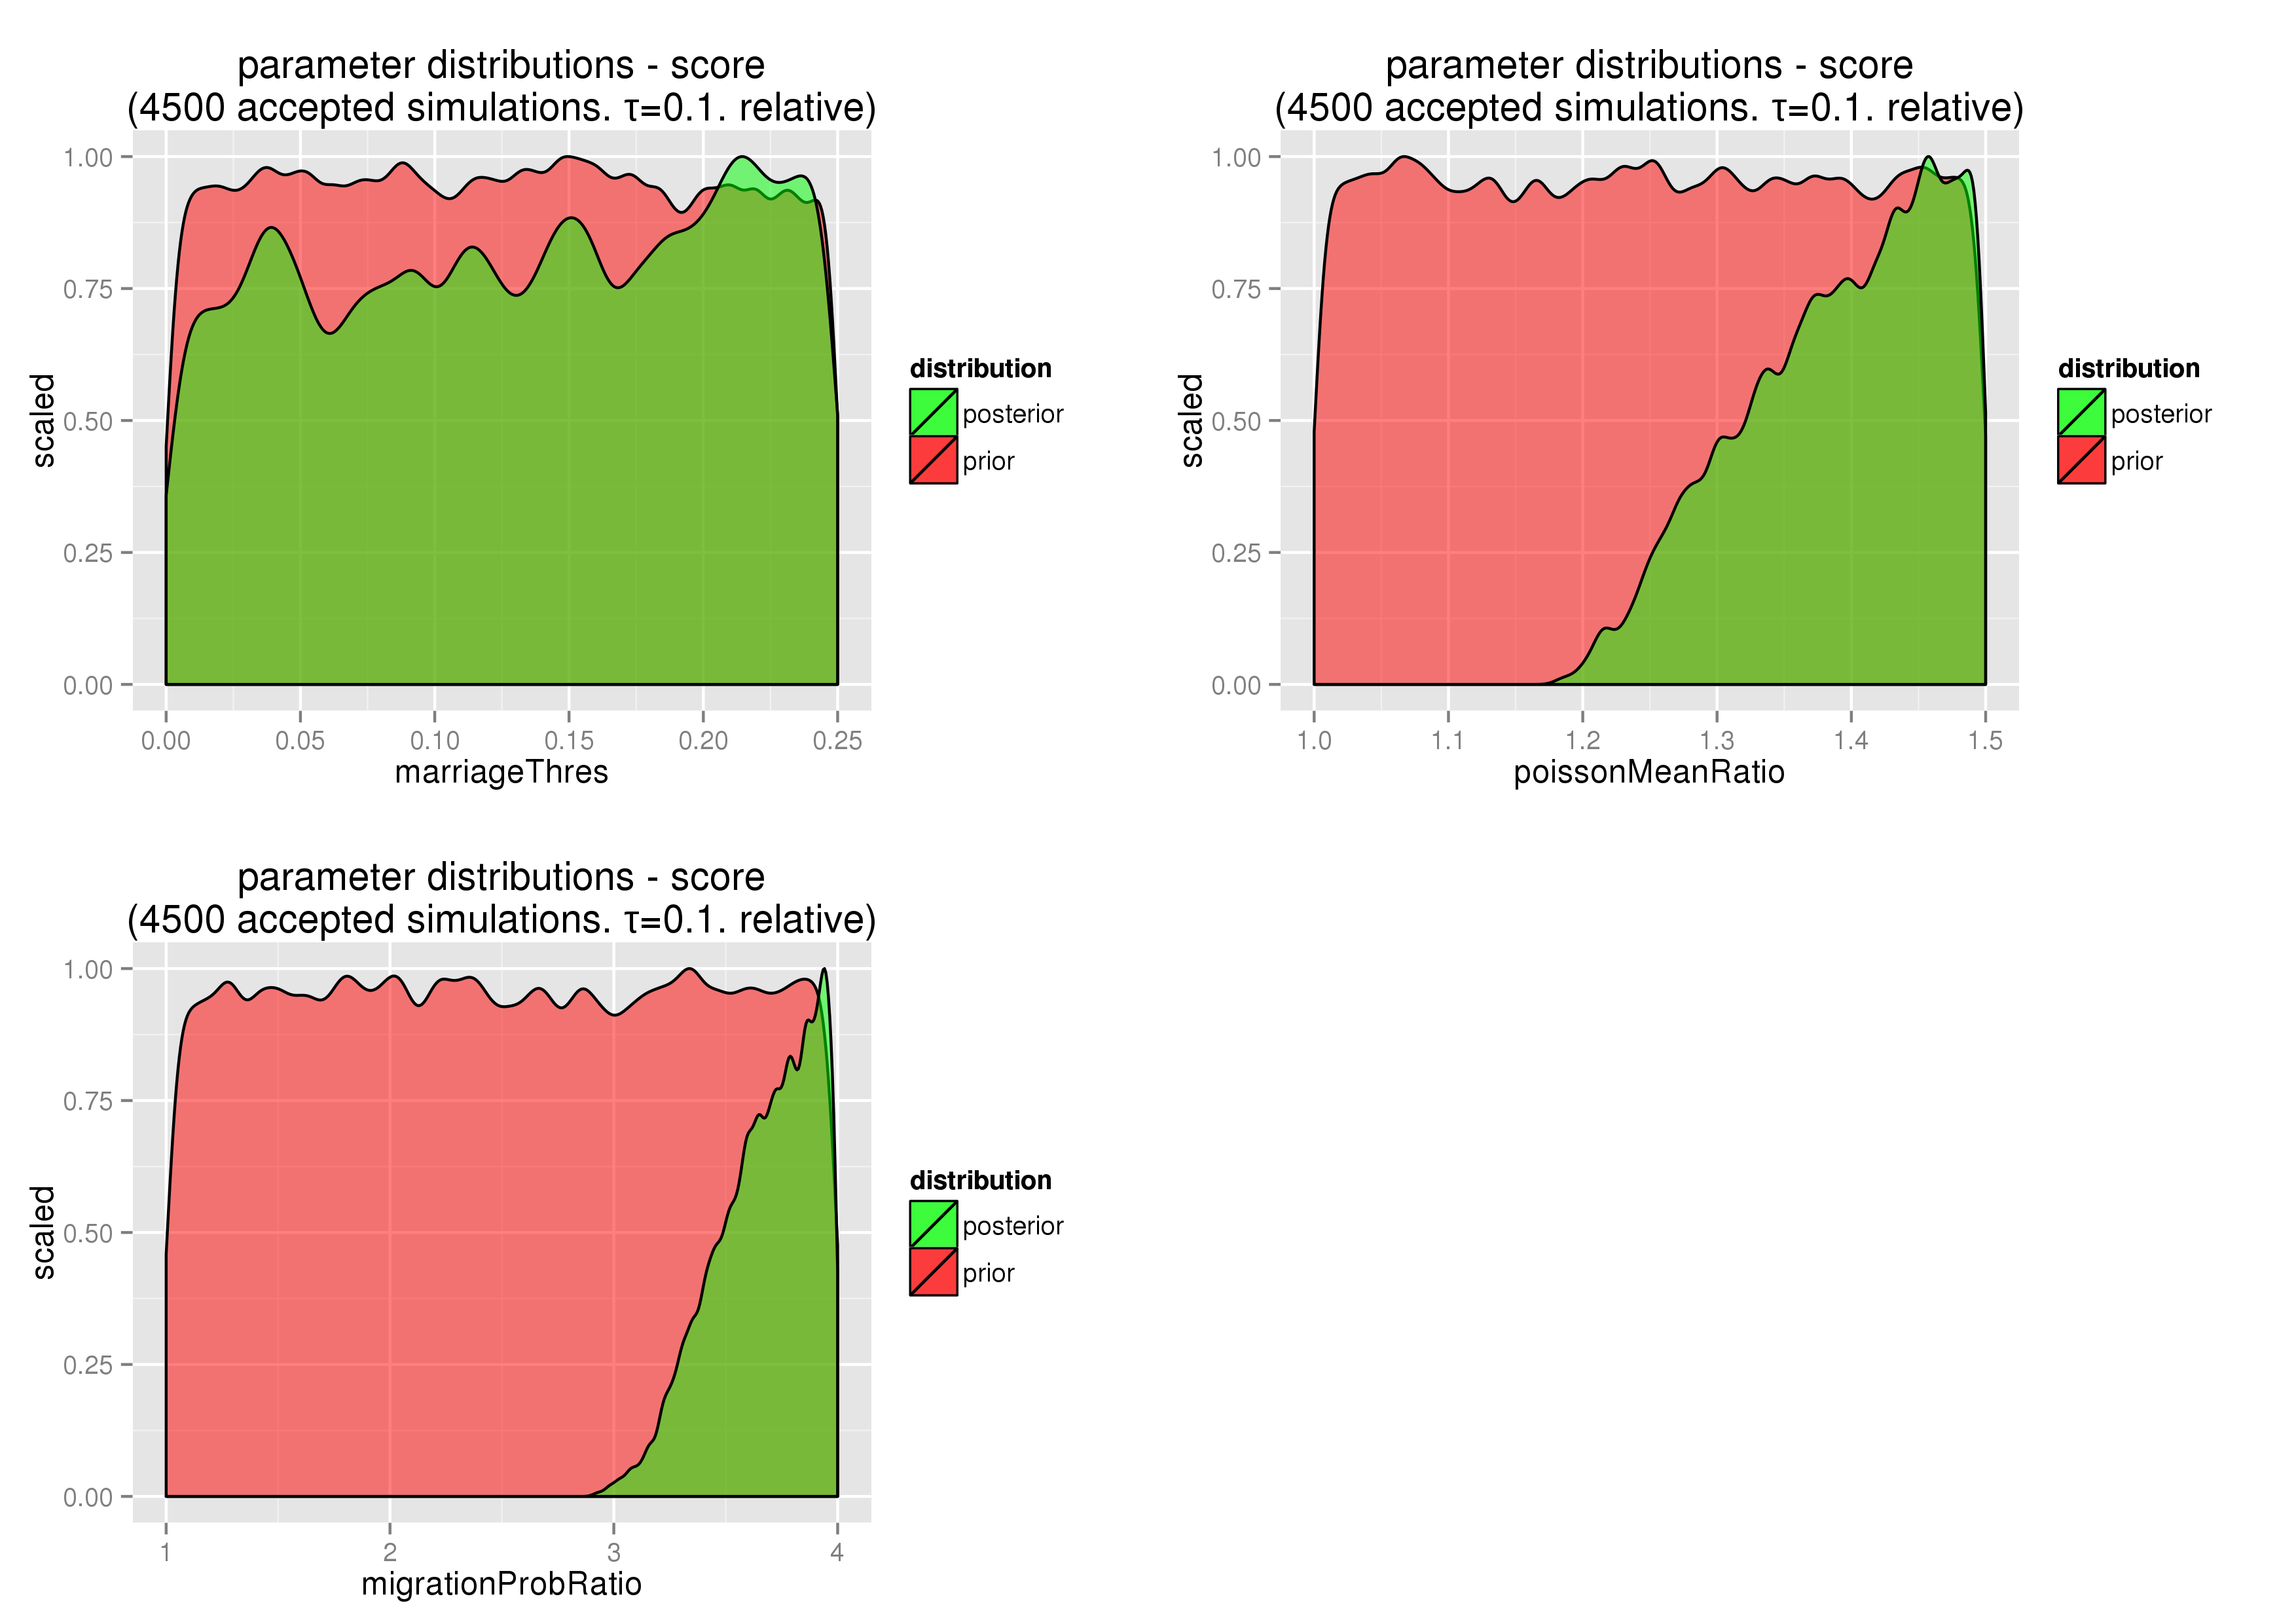
\includegraphics[width=1\textwidth]{../data/abc-priors-posteriors.png}
	\caption{Prior and posterior distributions for an ABC analysis.}
	\label{abc-prior-posterior}
\end{figure}

The implementation of the ABC framework being the last part of the internship, more useful results are to be expected in the future when more ABCs will be run.

\chapter*{Conclusion}
\addcontentsline{toc}{chapter}{Conclusion}
The model used until is still undergoing changes, with the aim to make it more accurate and to take into account more factors.
The problem would be to add enough complexity to keep the model relevant while still being computationally simple enough so that it can be run in an acceptable amount of time.
Several aspects can be changed, ranging from the structure of agents and how they are managed in the model, to higher level tasks like the integration of resource management at different scales of the model to try to be more accurate and have more realistic behaviours.

This project will continue evolving and the work done until now will still be useful.
The scripts written will still be able to handle the data output by the model, and even if the data changes, only slight changes will be necessary for them to continue working.

On an anthropological level, results have already been found.
Even if research needs to be followed-up, the first findings have been able to discard some scenarios and to confirm others.
For example, the marriage bias has been confirmed.
Indeed, the simulations done without any bias or with an inverted bias were discarded by the ABC framework.
A trade-off between fecundity and migration rate has also been shown, meaning that a good parameter set can either have high fecundity but low migration rate, high migration rate and low fecundity, or medium values for these two parameters.
Any of these combinations yields simulations whose final state is similar to the real values observed in the field.

This internship has been an opportunity to work on a real research problem, to think about it and to decide what approach would be best to answer the questions raised by this problem.
In order to do so, different pieces of software have been developed and will be reusable to continue the research in the same direction.
The languages of the different scripts have been chosen to use the ones adapted to a specific task; for example all the heavy data handling has been done in R.
The code produced aims to easily handle the data generated by the model used for this project and to represent it in a way that conclusions can be made by looking at the visualisations of the data and not having to manually analyse the huge quantity of data generated by the numerous iterations of the model.
All the data have been handled in a recent but recognised statistical context, an ABC framework, that guarantees that the interpretations made are not biased and can be found again using other implementations of the same statistical framework.

\newpage

\glossarystyle{altlist}
\printglossaries
\addcontentsline{toc}{chapter}{Glossary}


\bibliography{main_v2}
\bibliographystyle{apalike}
\addcontentsline{toc}{chapter}{Bibliography}

\appendix
% change section numbering to roman numbers
\renewcommand{\thesection}{\Roman{section}}
\addtocontents{toc}{\protect\setcounter{tocdepth}{0}}
% example visualisations
%\addtocontents{toc}{\setcounter{tocdepth}{-1}}
\chapter{Examples of visualisation}
\label{app:ex-visu}
%\addtocontents{toc}{\protect\setcounter{tocdepth}{0}}

This appendix presents different visualisation examples that are generated by the developed scripts.

\section{Stability}
\begin{figure}[H]
	\centering
	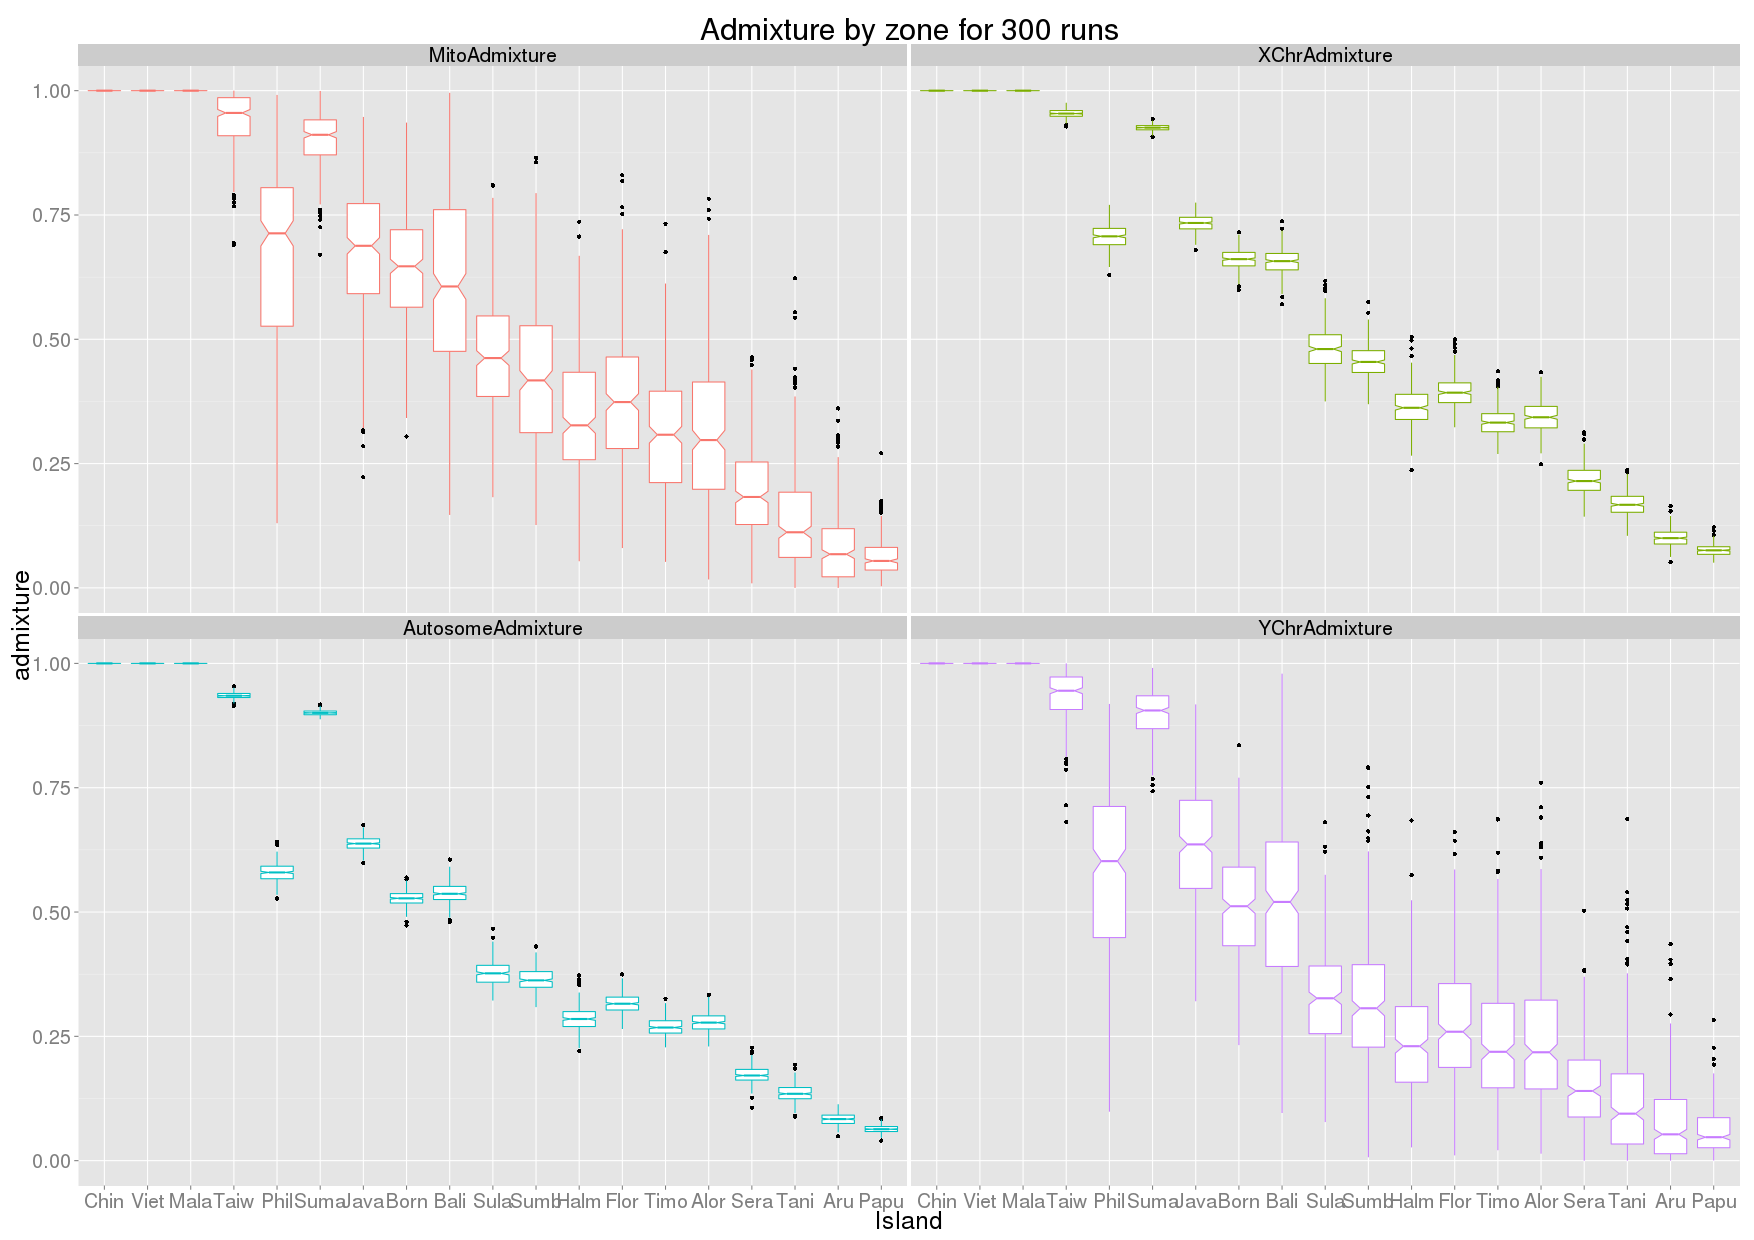
\includegraphics[scale=0.2]{../data/stability.png}
	\caption{Box-plots of admixture by island, separated by type of DNA.}
	\label{app:stability}
\end{figure}

\section{Sensitivity}
\begin{figure}[H]
	\centering
	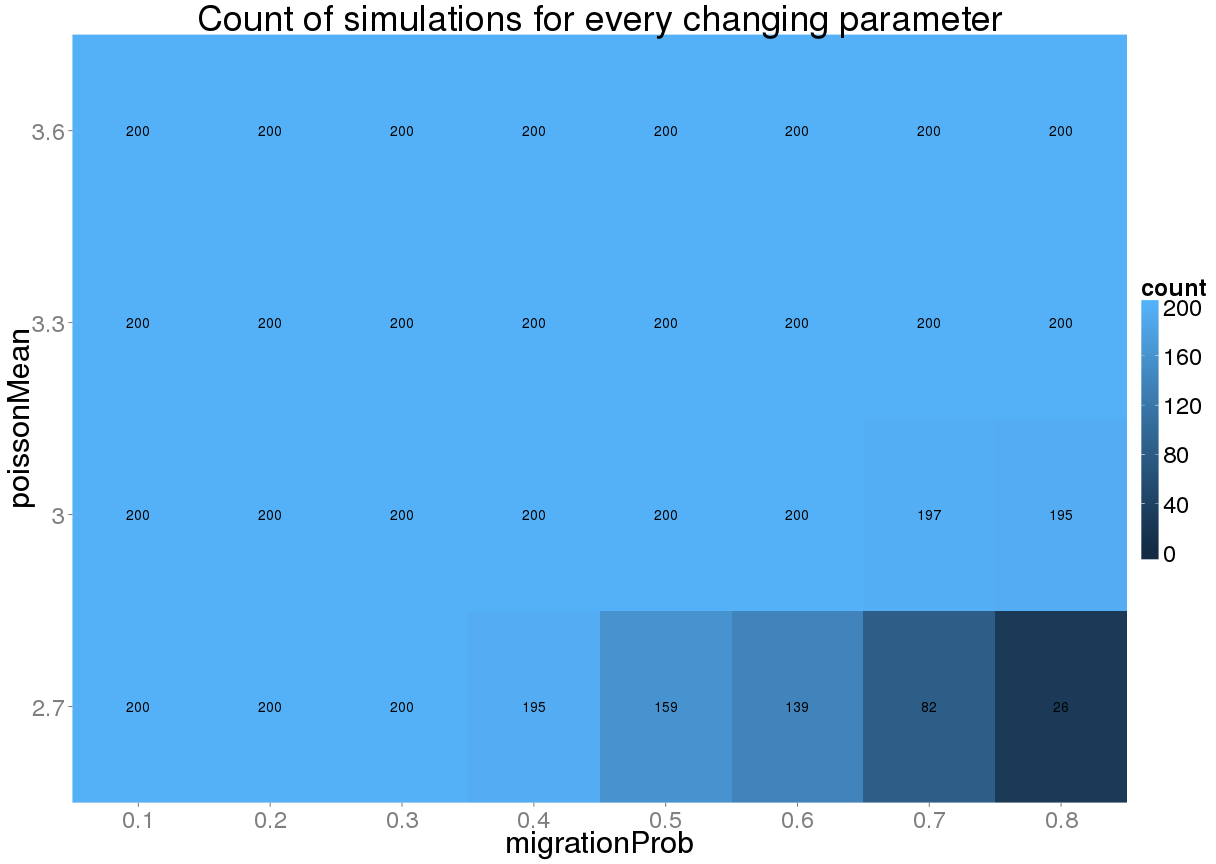
\includegraphics[scale=0.26]{../data/count-2d.png}
	\caption{Heat-map of counts of simulations for a one-dimensional sweep of migrationProb and poissonMean values. Failed simulations are revealed for both high migrationProb and low poissonMean values (dark boxes).}
	\label{app:count-2d}
\end{figure}

\begin{figure}[H]
	\centering
	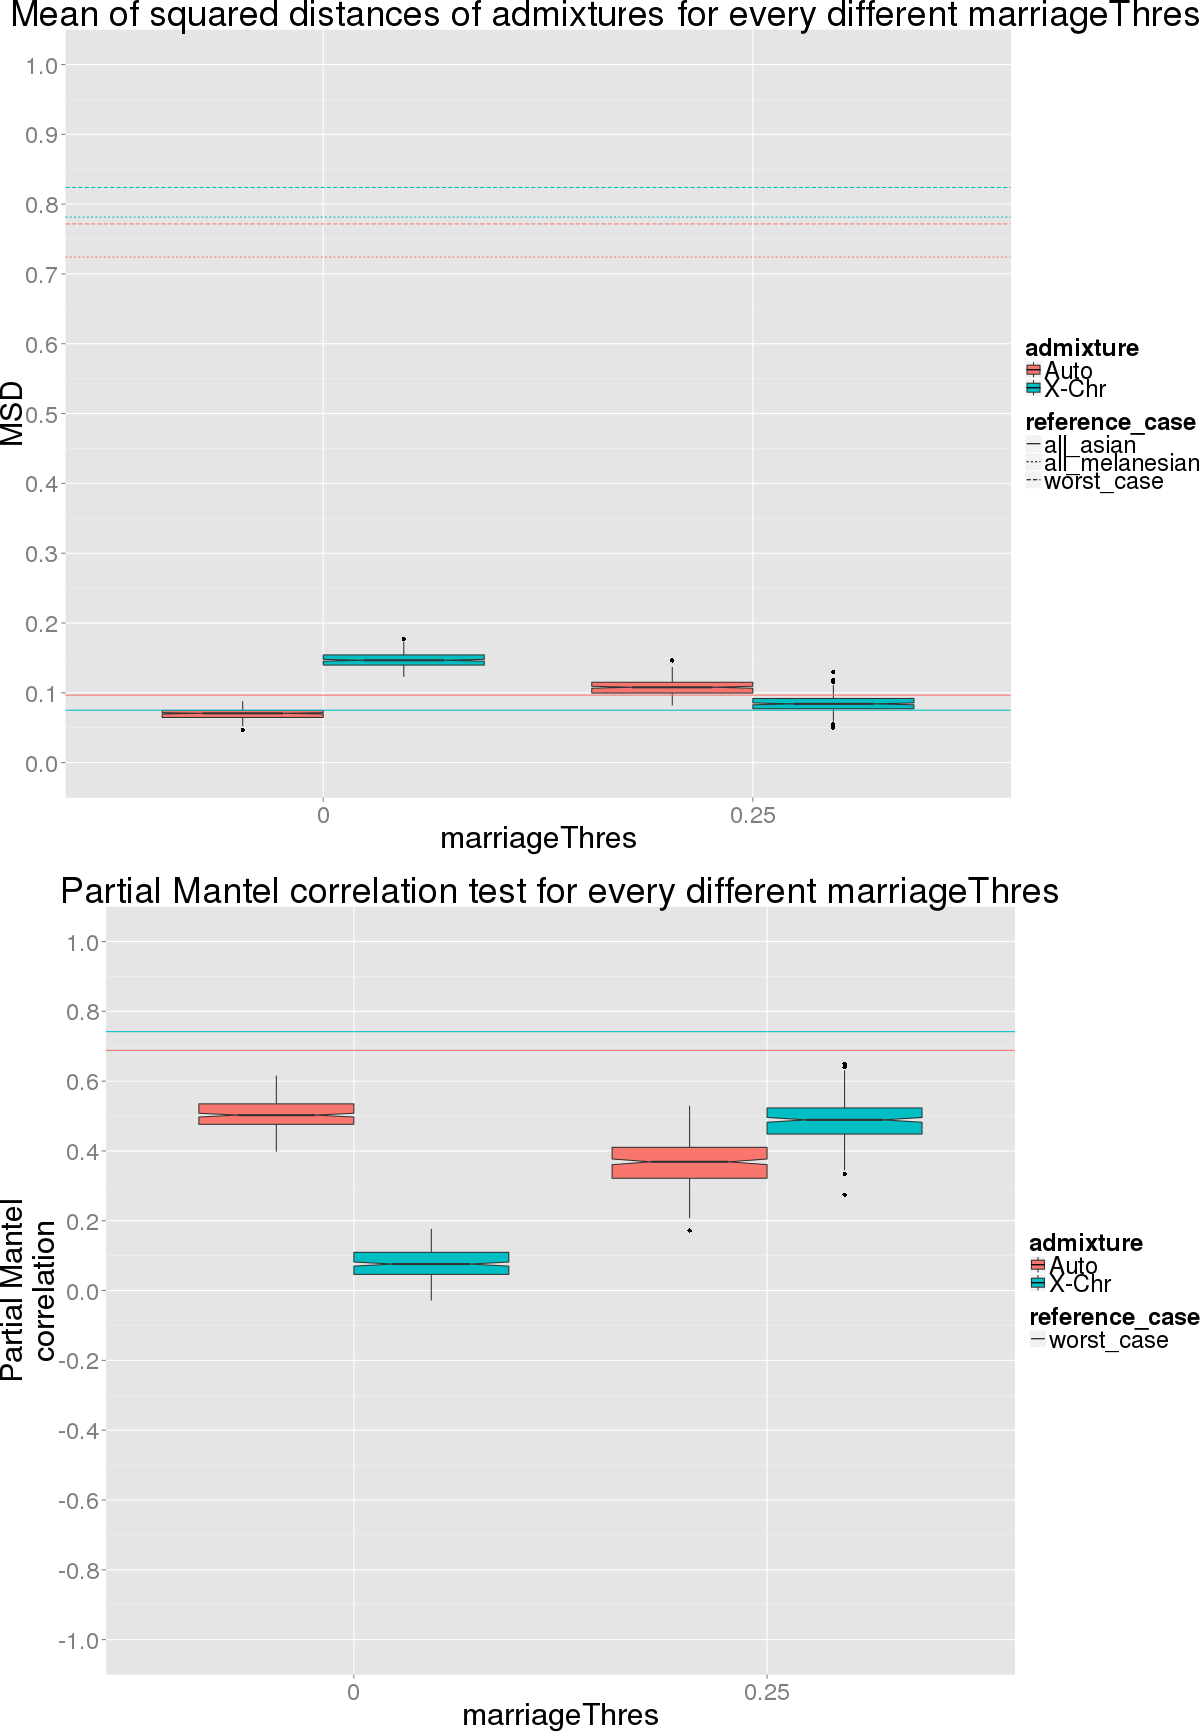
\includegraphics[scale=0.31]{../data/sensit-comp-1d.png}
	\caption{Box-plots of comparisons of simulations vs. real data for a one-dimensional sweep of marriageThres values. Additional lines corresponding to pre-defined extreme reference cases.}
	\label{app:sensit-comp-1d}
\end{figure}

\begin{figure}[H]
	\centering
	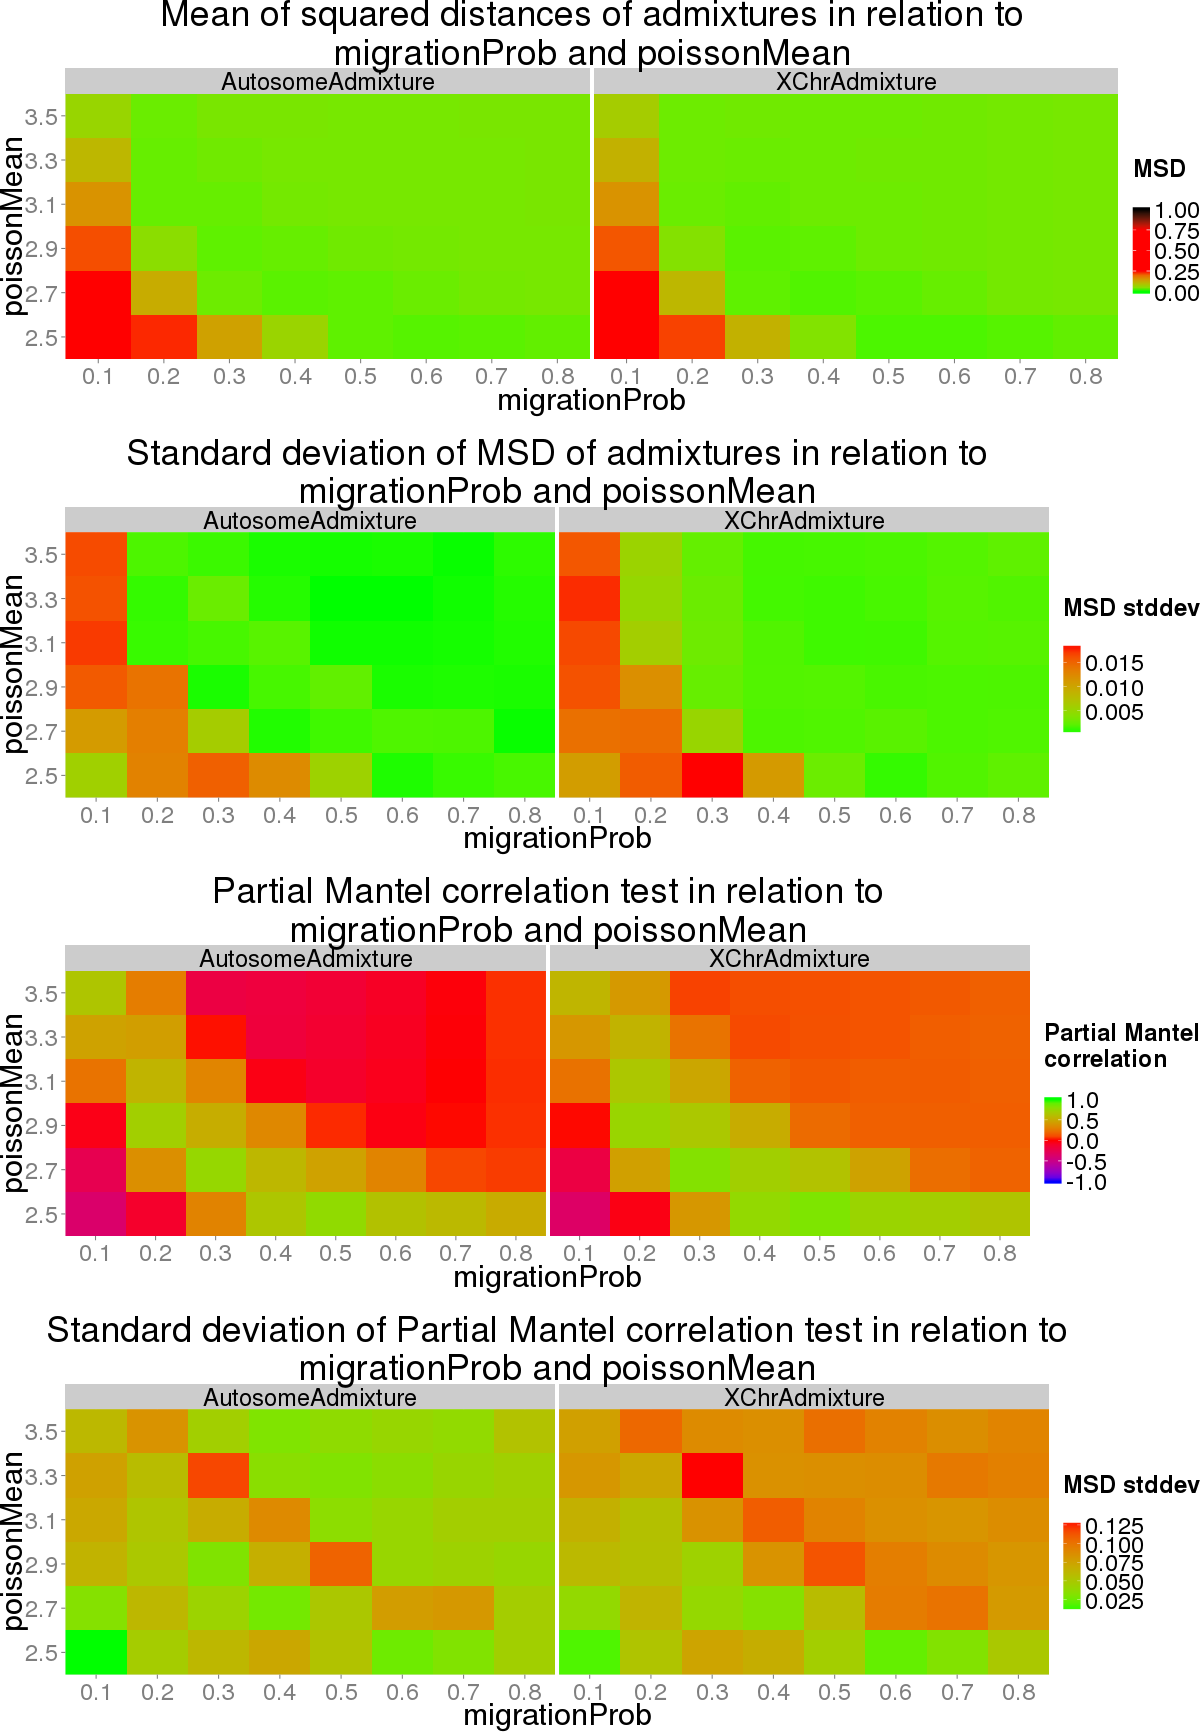
\includegraphics[scale=0.31]{../data/sensit-comp-2d.png}
	\caption{Heat-maps of comparisons and corresponding standard deviations of simulations vs. real data for a two-dimensional sweep of migrationProb and poissonMean values.}
	\label{app:sensit-comp-2d}
\end{figure}


\chapter{Benchmarks}
\label{app:bench}

\section{Merging}
\begin{figure}[H]
	\centering
	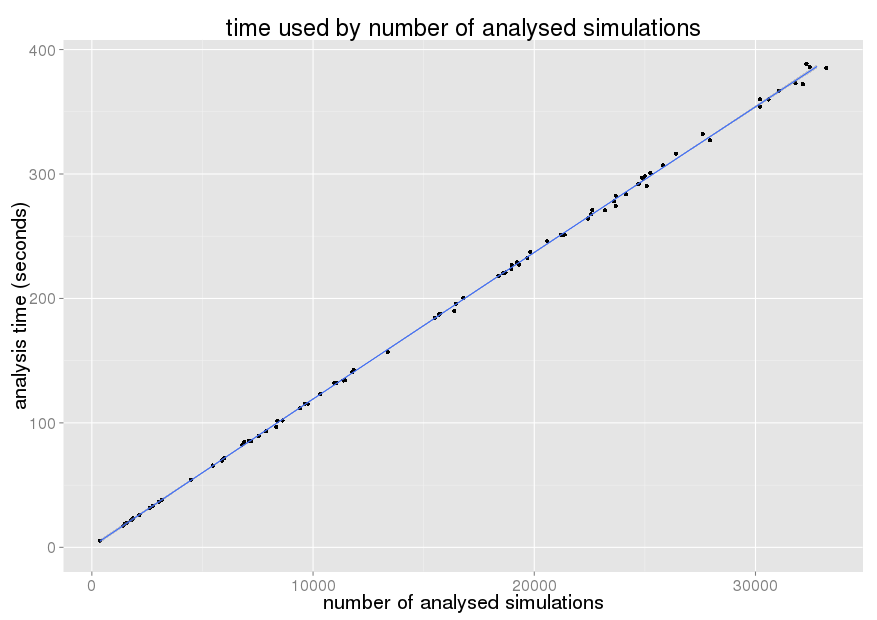
\includegraphics[scale=0.35]{../data/merge-timeByNSimulations.png}
	\caption{Time used by the scripts in relation to the number of simulations merged. Corresponding, in the work-flow, to \texttt{merge.R}.}
	\label{app:bench-merging-time}
\end{figure}

\begin{figure}[H]
	\centering
	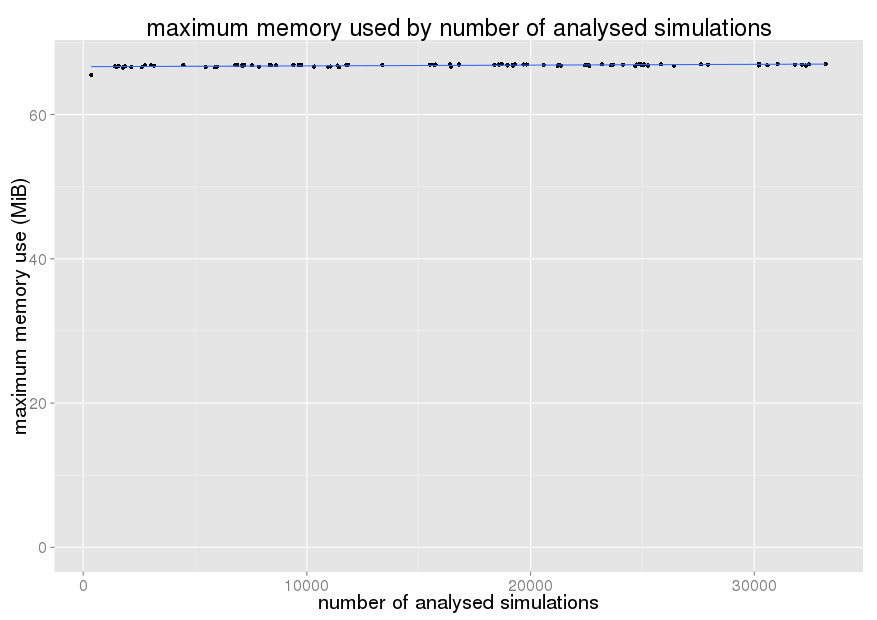
\includegraphics[scale=0.35]{../data/merge-maxMemByNSimulations.png}
	\caption{Maximum memory used by the scripts in relation to the number of simulations analysed. Corresponding, in the work-flow, to \texttt{merge.R}.}
	\label{app:bench-merging-mem}
\end{figure}


\section{Analysis}
note: update with latest changes (hopefully, better values)
\begin{figure}[H]
	\centering
	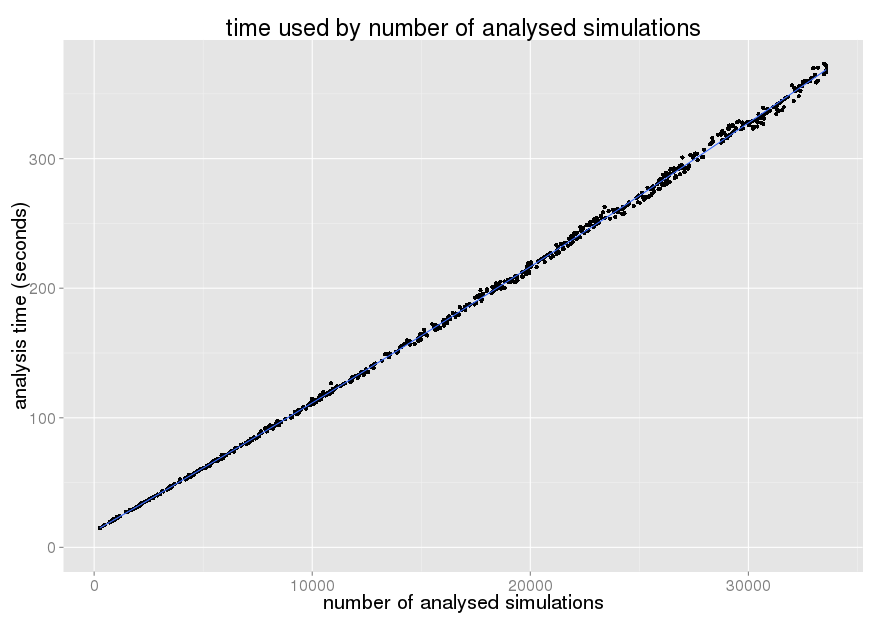
\includegraphics[scale=0.35]{../data/analysis-timeByNSimulations.png}
	\caption{Time used by the scripts in relation to the number of simulations analysed. Corresponding, in the work-flow, to \texttt{analysis.R}, \texttt{sensitivity.R} and the creation of the corresponding output files.}
	\label{app:bench-analysis-time}
\end{figure}

\begin{figure}[H]
	\centering
	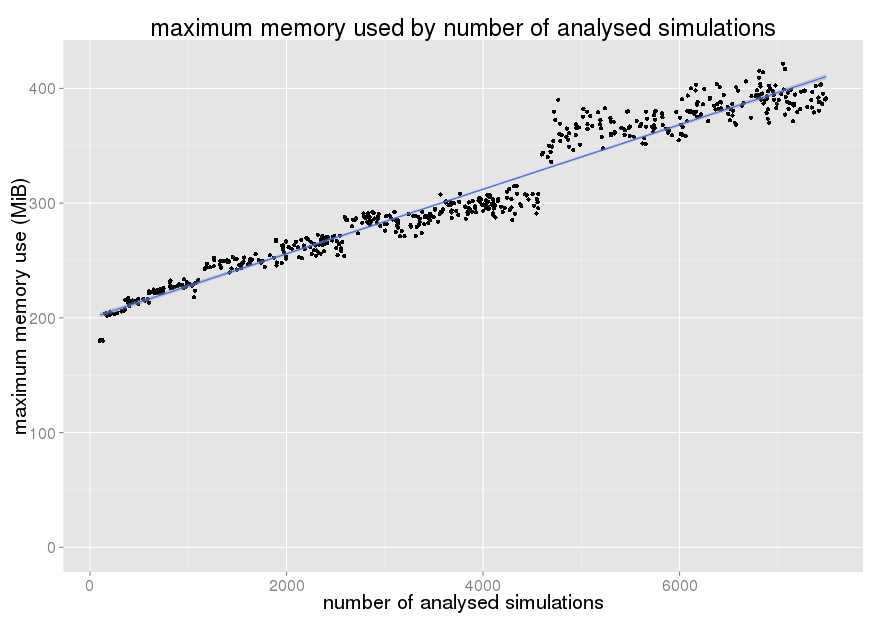
\includegraphics[scale=0.35]{../data/analysis-maxMemByNSimulations.png}
	\caption{Maximum memory used by the scripts in relation to the number of simulations analysed. Corresponding, in the work-flow, to \texttt{analysis.R}, \texttt{sensitivity.R} and the creation of the corresponding output files.}
	\label{app:bench-analysis-mem}
\end{figure}

% overview

\end{document}


